\documentclass{article}
\usepackage[utf8]{inputenc}
\usepackage{graphicx}
\title{TUGAS RESUME}
\author{Gany Berdu Sura - 1184008 }
\date{November 2019}

\begin{document}

\maketitle

\section{CARA MEMBUAT APLIKASI BUILDER DENGAN FILE EXCEL} 
\begin{enumerate}
    \item bukalah oracle apec dan masuk dengan menggunakan akun yang telah terdaftar seperti dibawah ini
    \begin{center}
    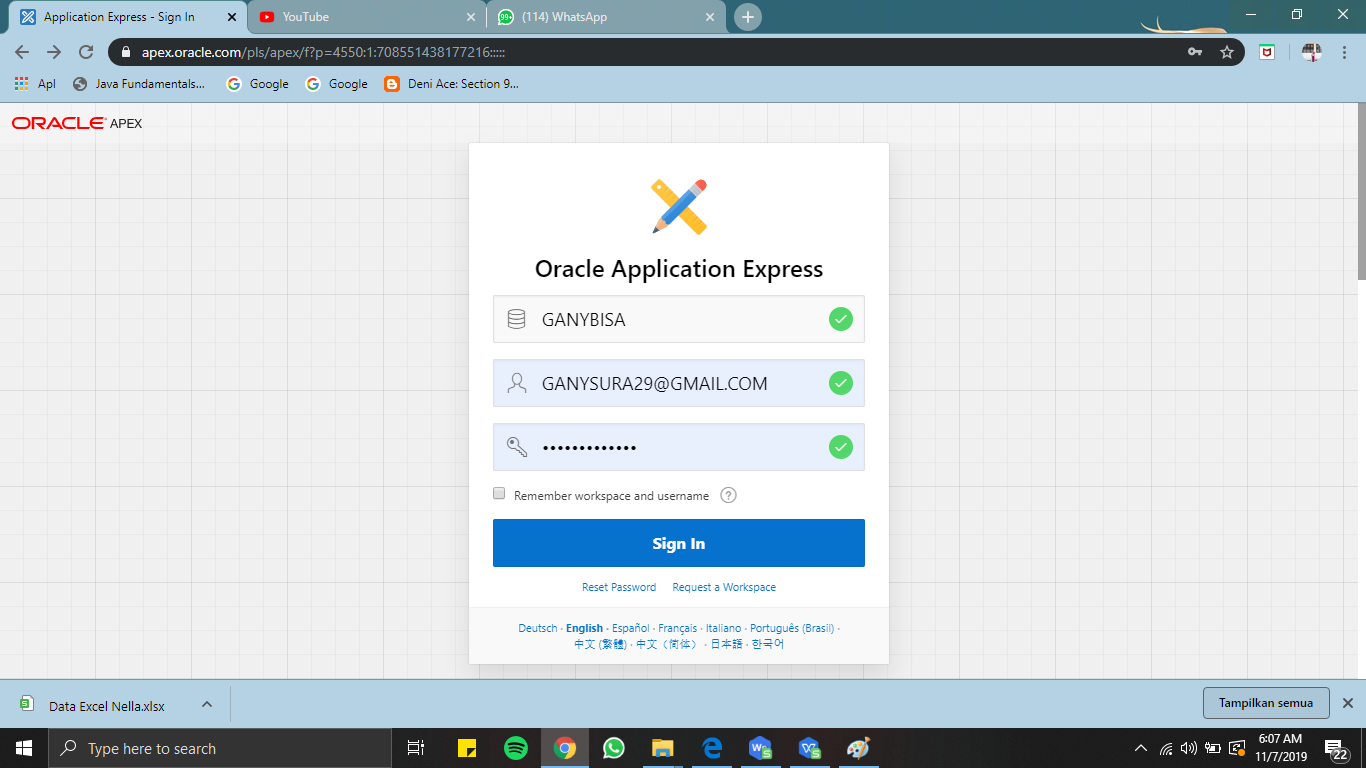
\includegraphics[width=.6\textwidth]{gambar/1.png}
    \end{center}
    \item kemudian pilih create dan pilih from file
    \begin{center}
    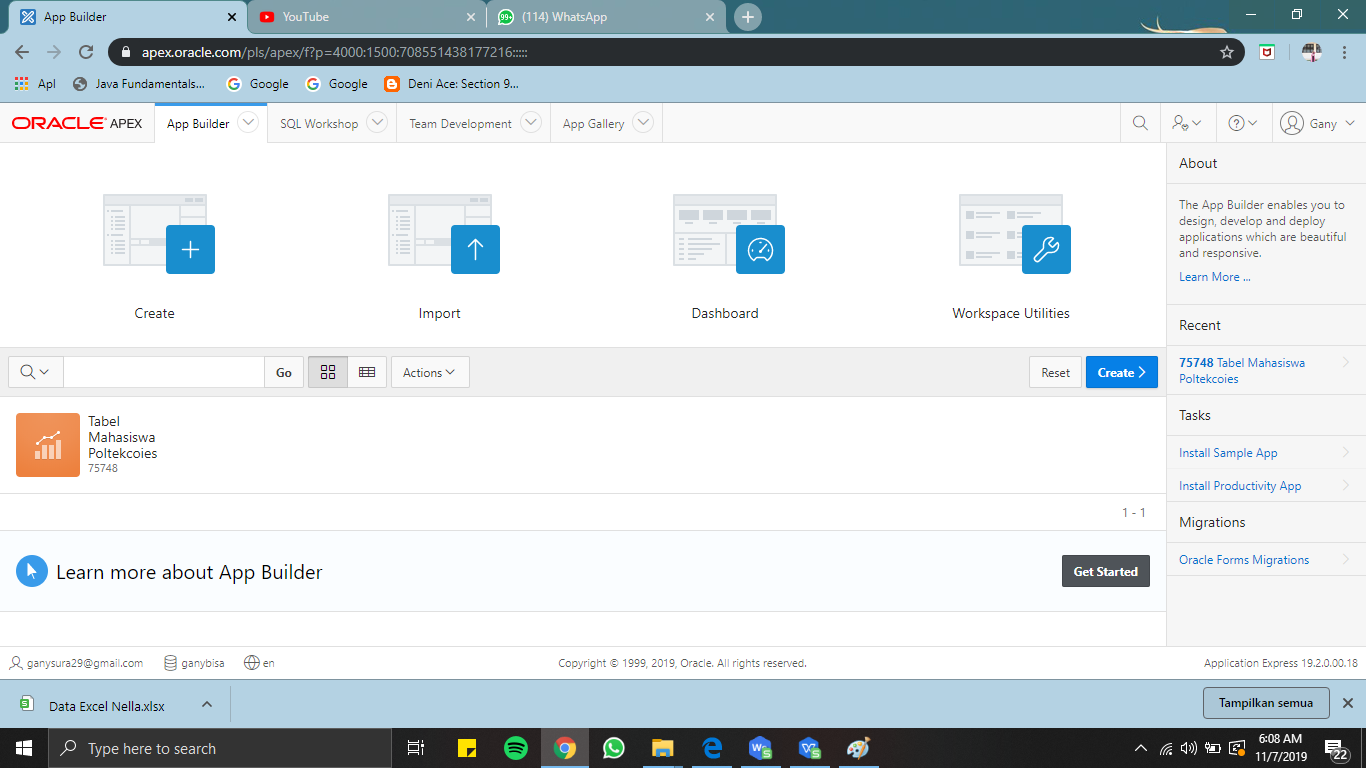
\includegraphics[width=.6\textwidth]{gambar/2.png}
    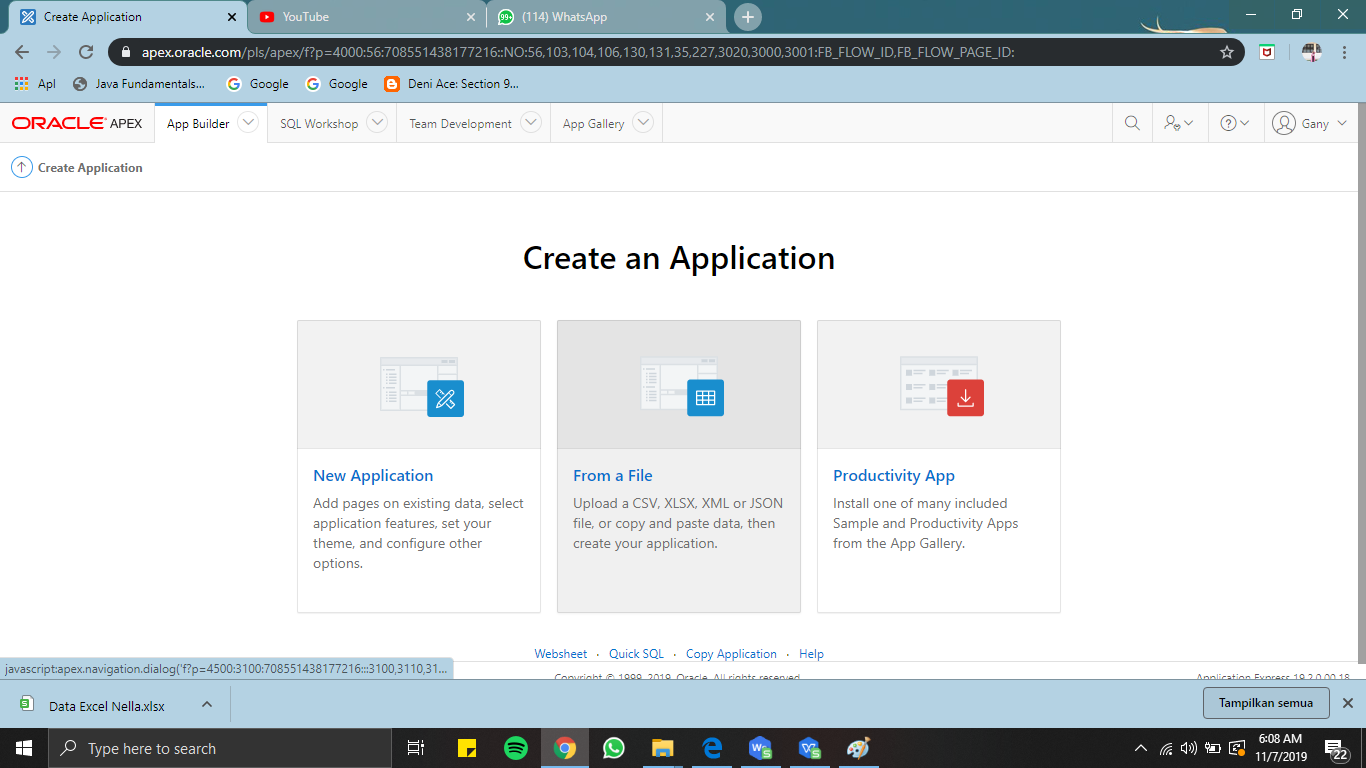
\includegraphics[width=.6\textwidth]{gambar/3.png}
    \end{center}
    \item setelah terbuka maka drag file excel yang telah dibuat
    \begin{center}
    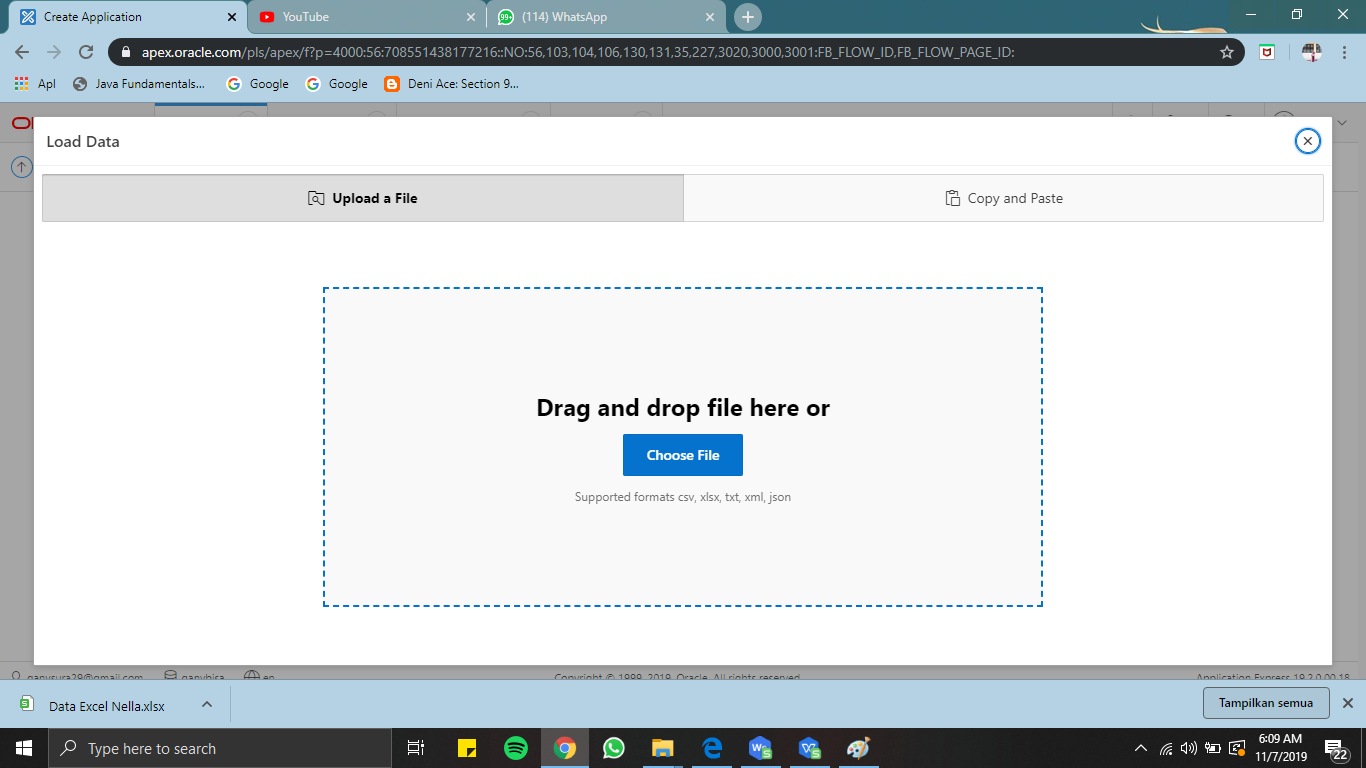
\includegraphics[width=.6\textwidth]{gambar/4.png}
    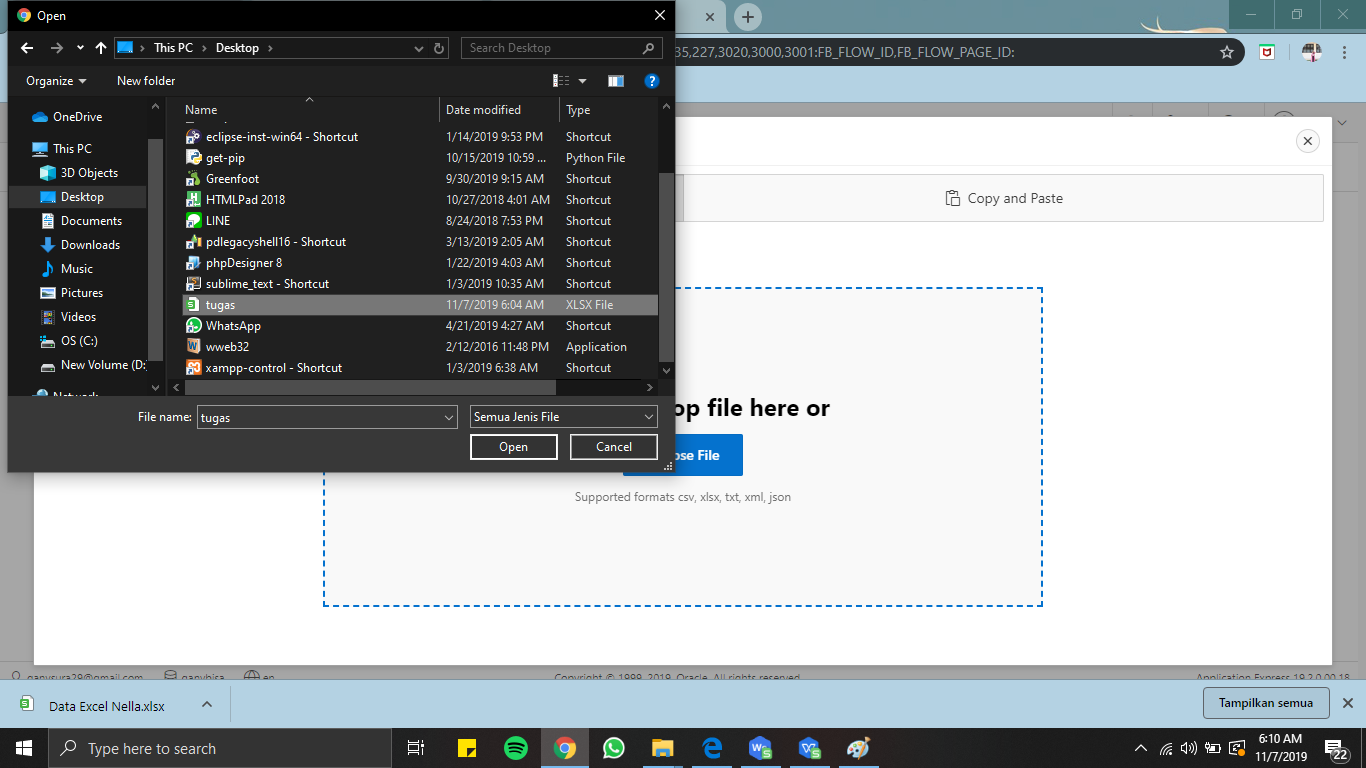
\includegraphics[width=.6\textwidth]{gambar/5.png}
    \end{center}
    \item kemudian setelah terbuka ganti nama tabel dan sesuaikan dengan tabel setiap data, kemudian create
    \begin{center}
    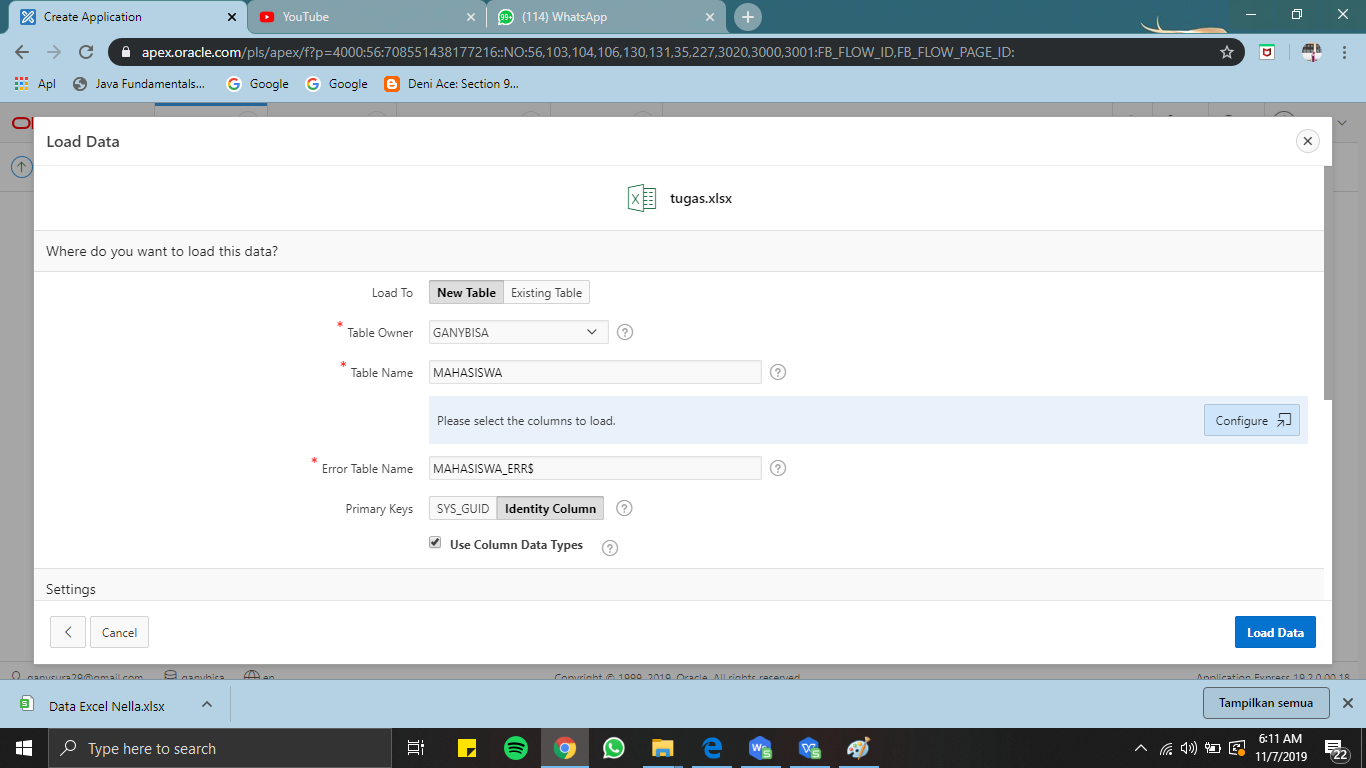
\includegraphics[width=.6\textwidth]{gambar/6.png}
    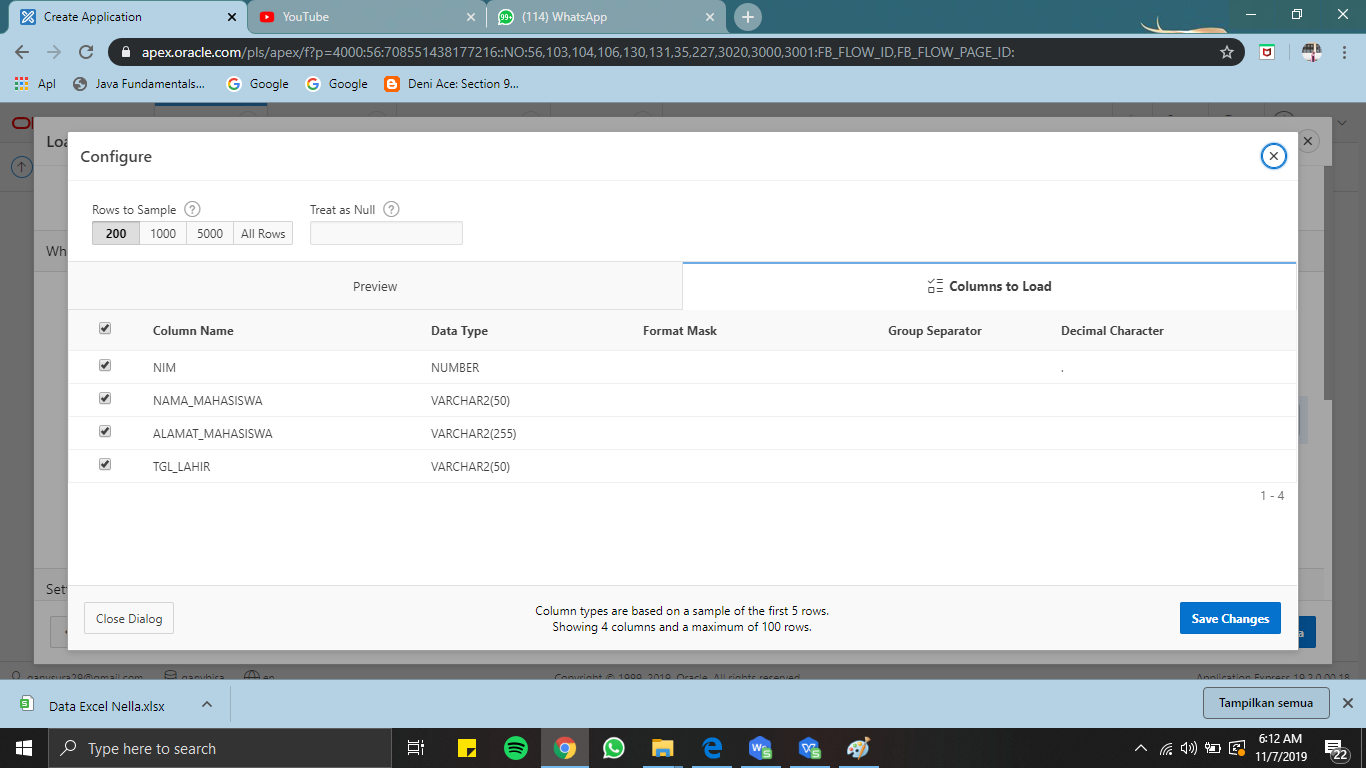
\includegraphics[width=.6\textwidth]{gambar/7.png}
    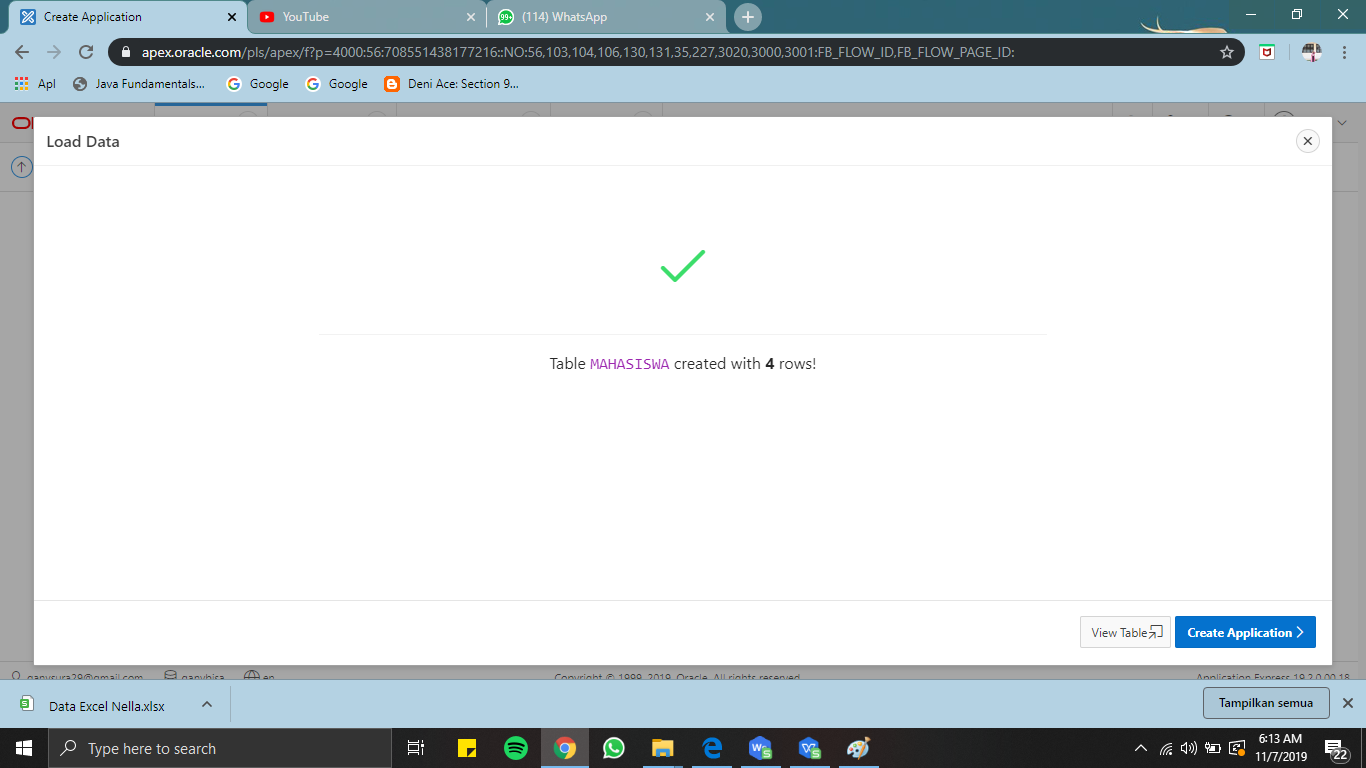
\includegraphics[width=.6\textwidth]{gambar/8.png}
    \end{center}
    \item lakukan hal yang sama untuk ke 5 data yang ada pada excel, seperti JADWAL,NILAI,DOSEN,KULIAH
    \begin{center}
    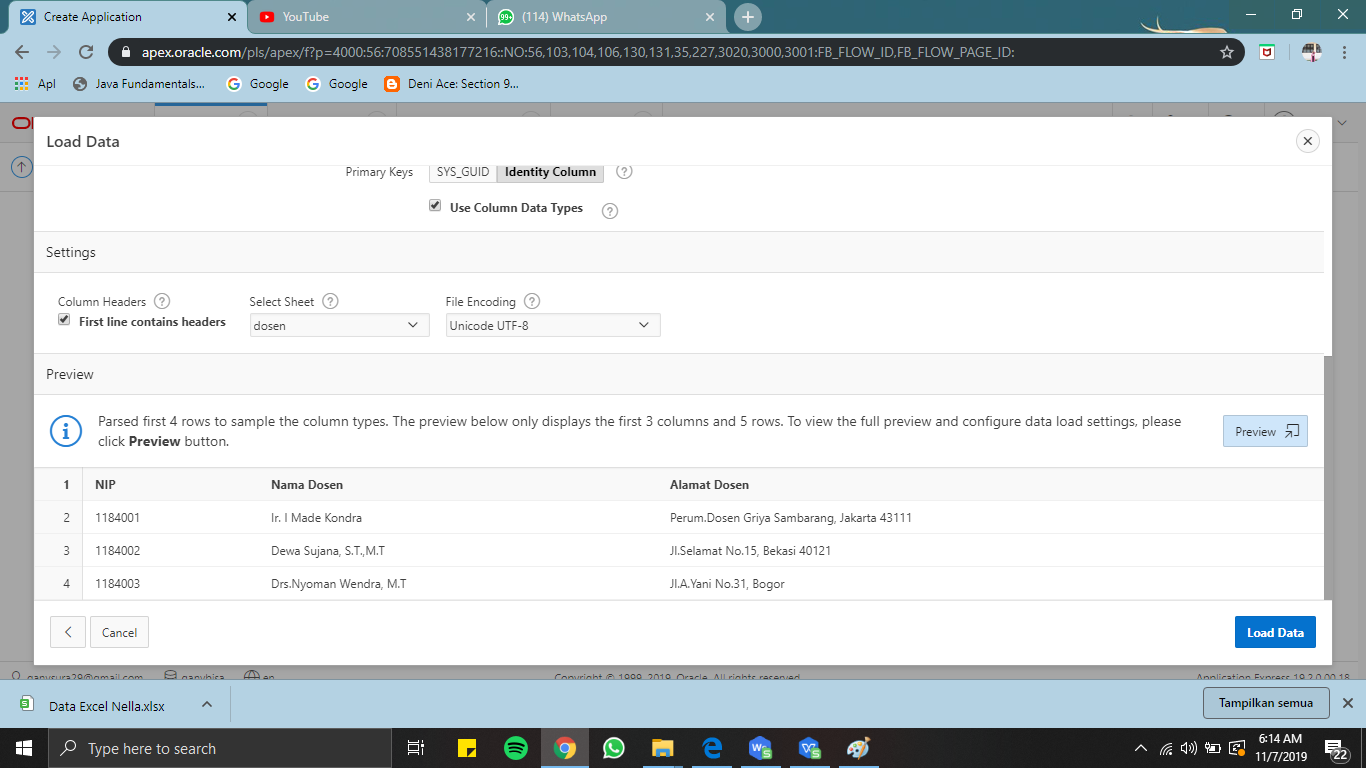
\includegraphics[width=.6\textwidth]{gambar/9.png}
    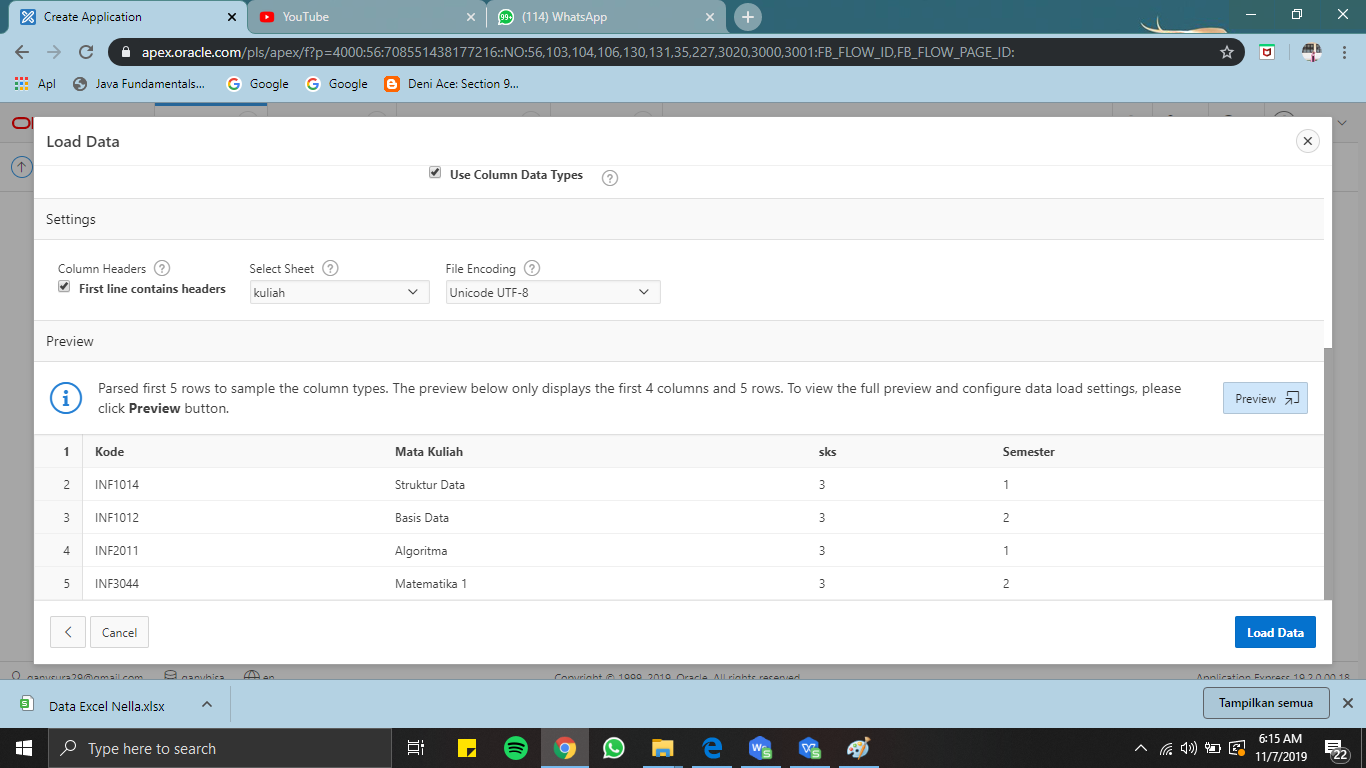
\includegraphics[width=.6\textwidth]{gambar/10.png}
    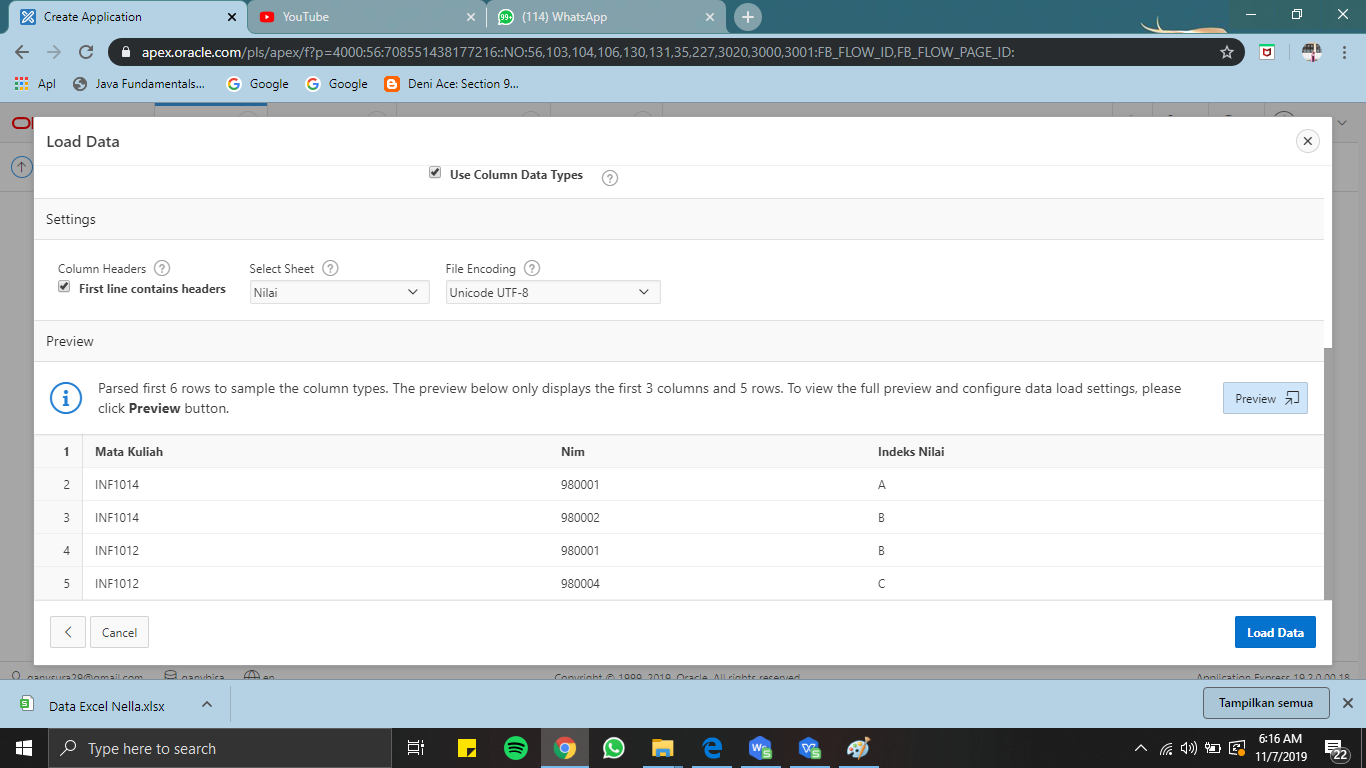
\includegraphics[width=.6\textwidth]{gambar/11.png}
    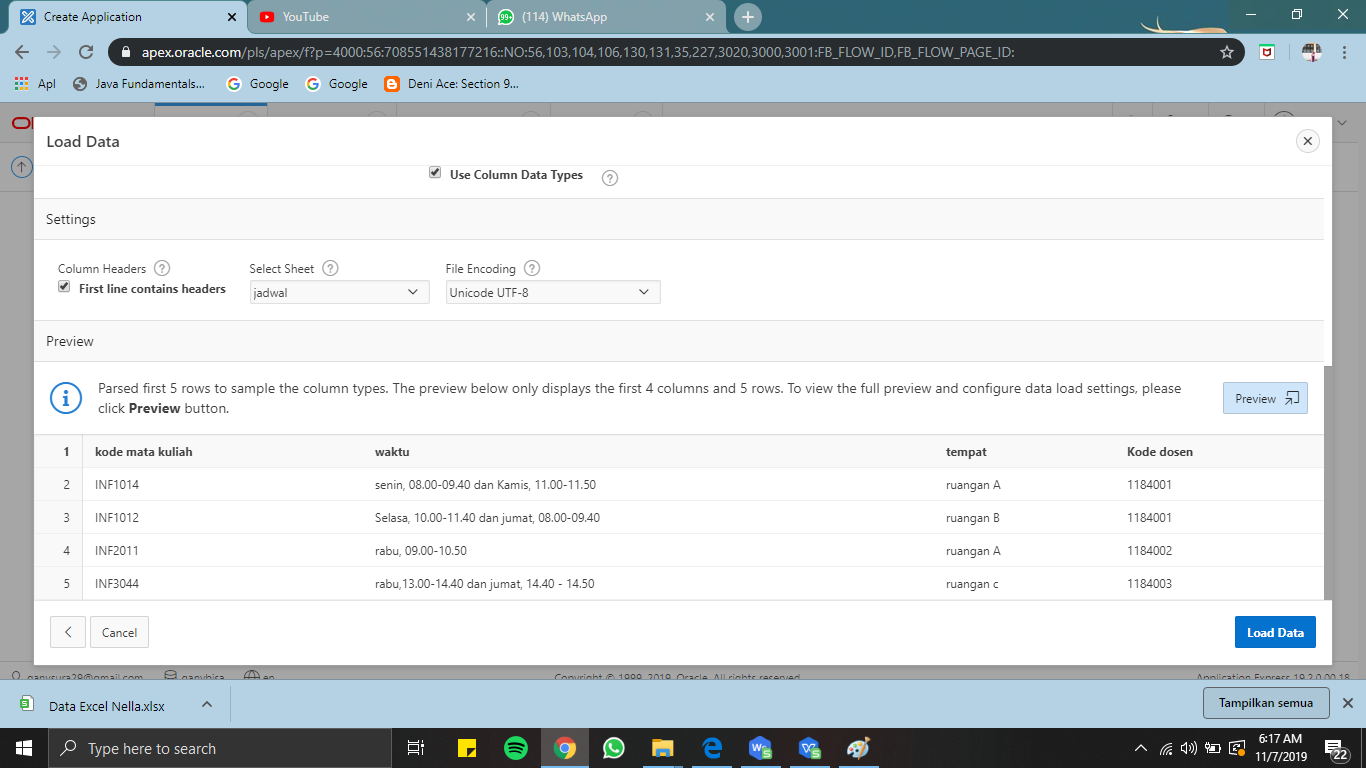
\includegraphics[width=.6\textwidth]{gambar/12.png}
    \end{center}
    \item setelah itu maka akan terbentuk 5 tabel
    \begin{center}
    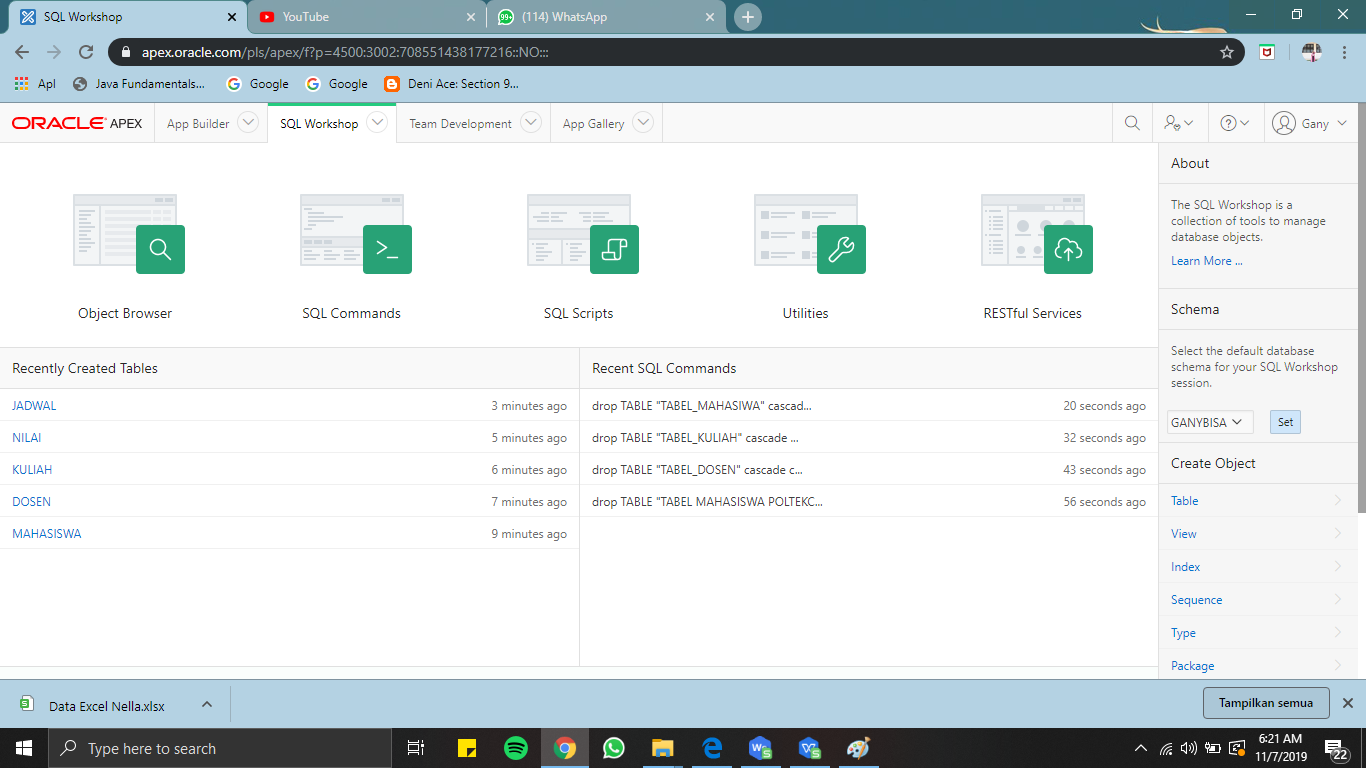
\includegraphics[width=.6\textwidth]{gambar/13.png}
    \end{center}
    \item setelah itu klik salah satu tabel, contohnya mahasiswa, dan setelah itu klik drop colom dan pilih dengan ID NUMBER dan kemudian next dan finish, lakukan kesemua tabel
    \begin{center}
    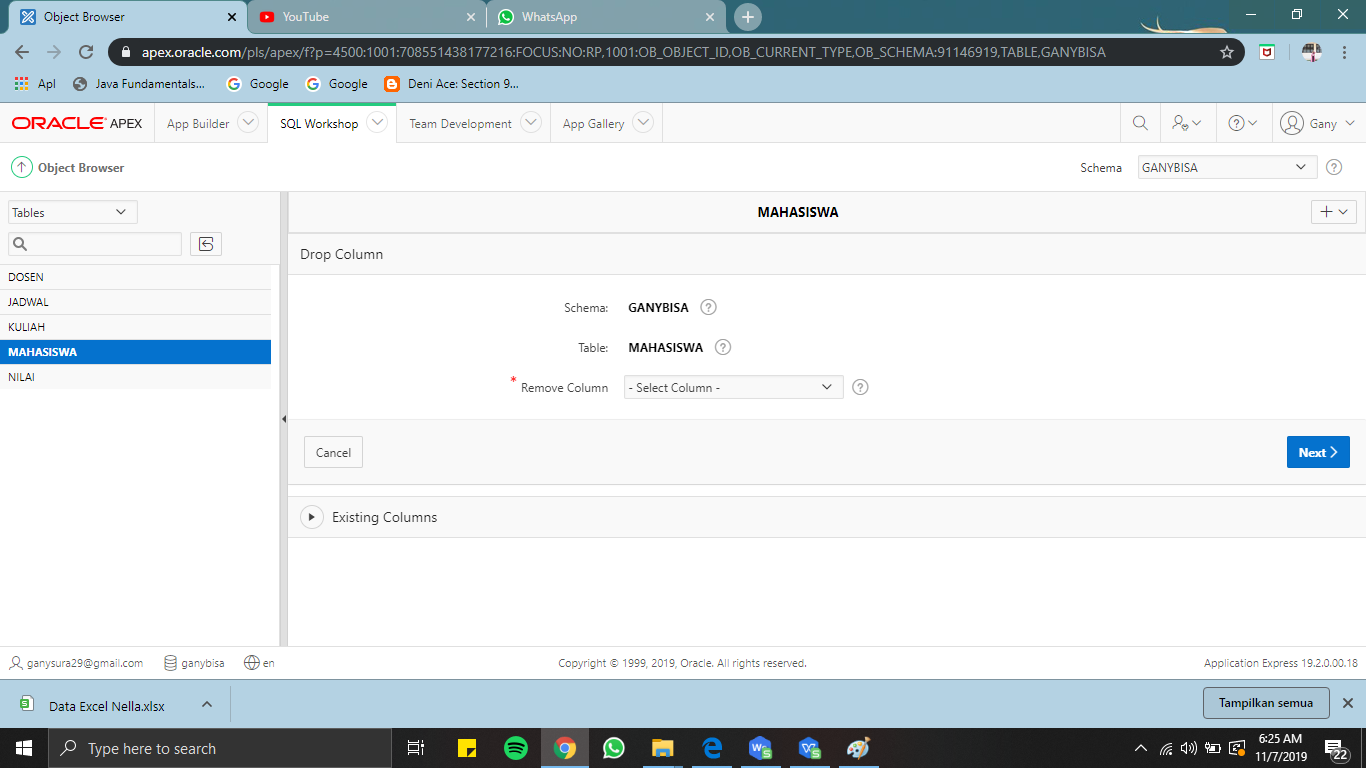
\includegraphics[width=.6\textwidth]{gambar/14.png}
    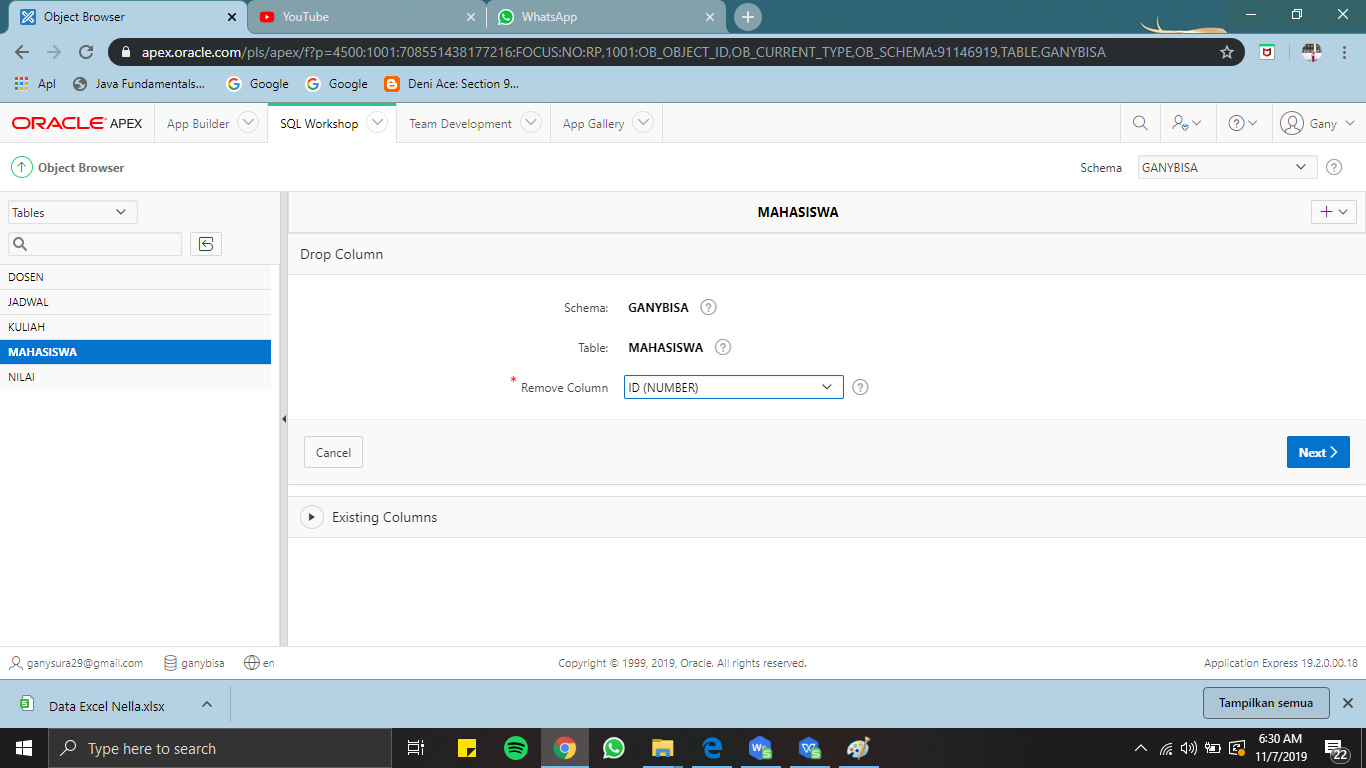
\includegraphics[width=.6\textwidth]{gambar/15.png}
    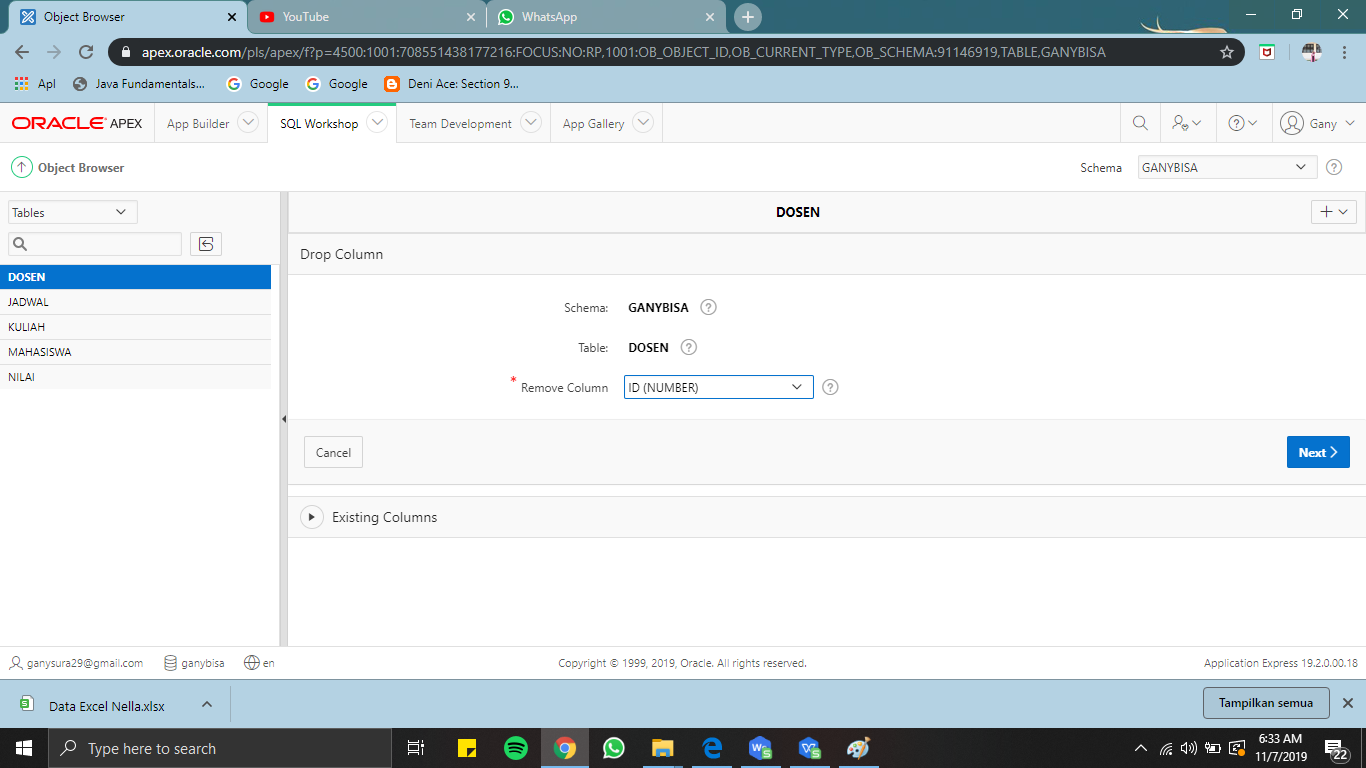
\includegraphics[width=.6\textwidth]{gambar/16.png}
    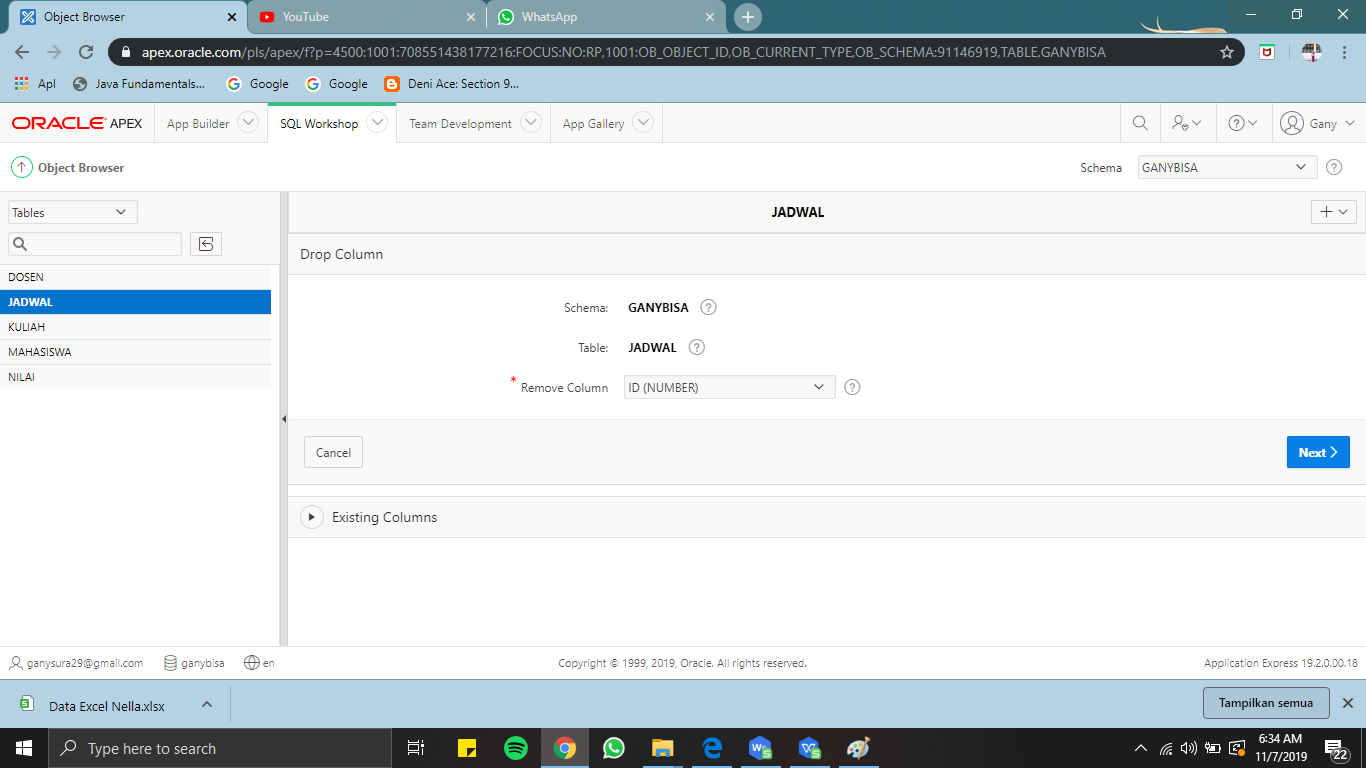
\includegraphics[width=.6\textwidth]{gambar/17.png}
    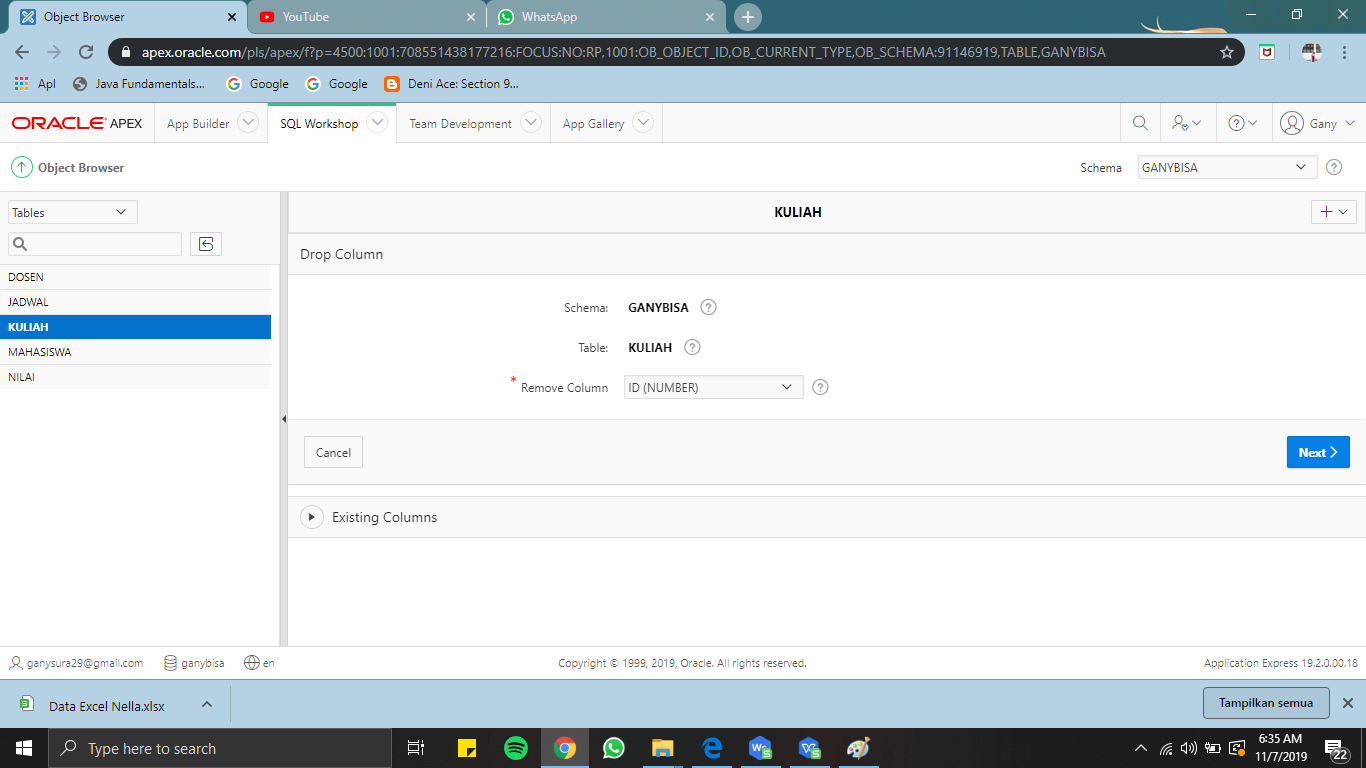
\includegraphics[width=.6\textwidth]{gambar/18.png}
    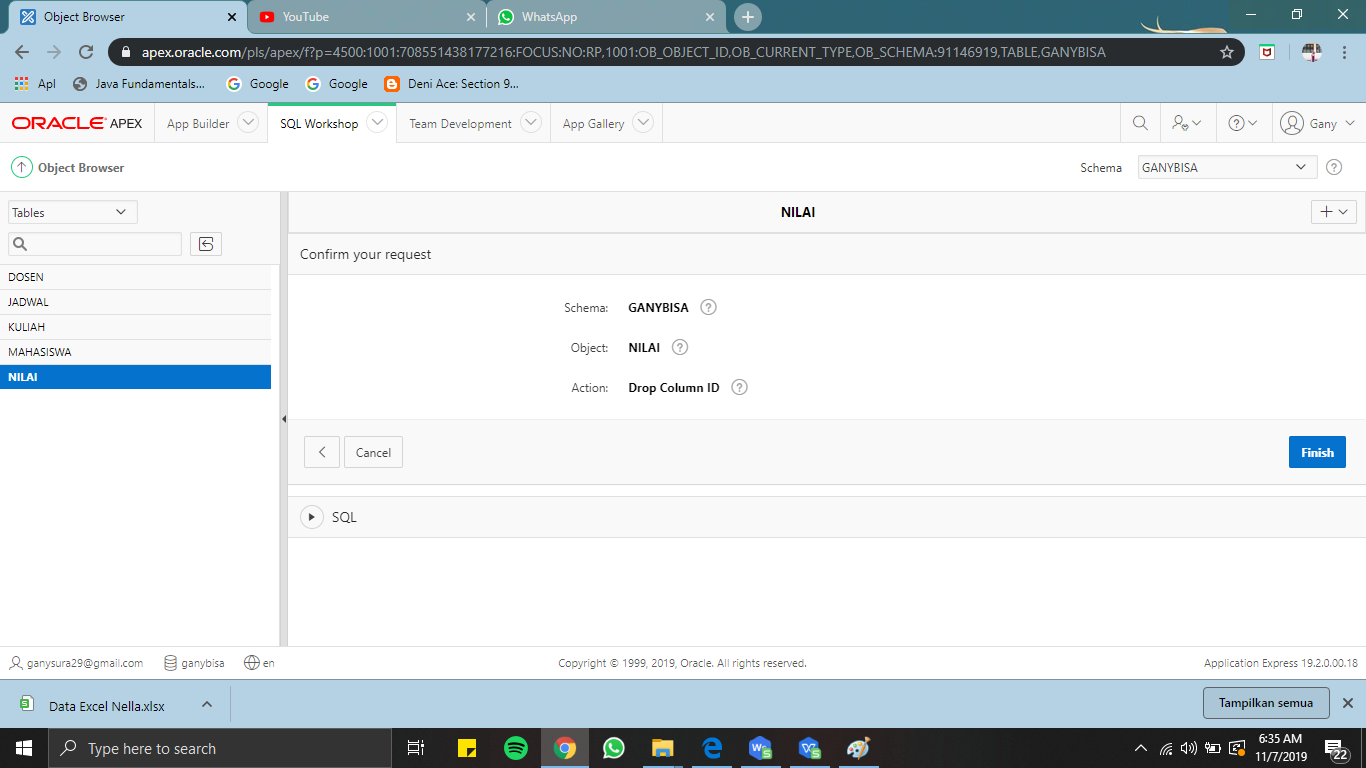
\includegraphics[width=.6\textwidth]{gambar/19.png}
    \end{center}
    \item setelah itu klik lagi salah satu tabel contoh mahasiswa, dan klik CONTRAINS dan create untuk membuat primary key , mari mulai dengan tabel mahasiswa, CONTAIN TYPE diganti menjadi PRIMARY KEY dan dan pilih tabel NIM , kemudian pilih tombol PLAY dan kita bisa lihat CODINGAN atau SQL yang langsung terbentuk
    \begin{center}
    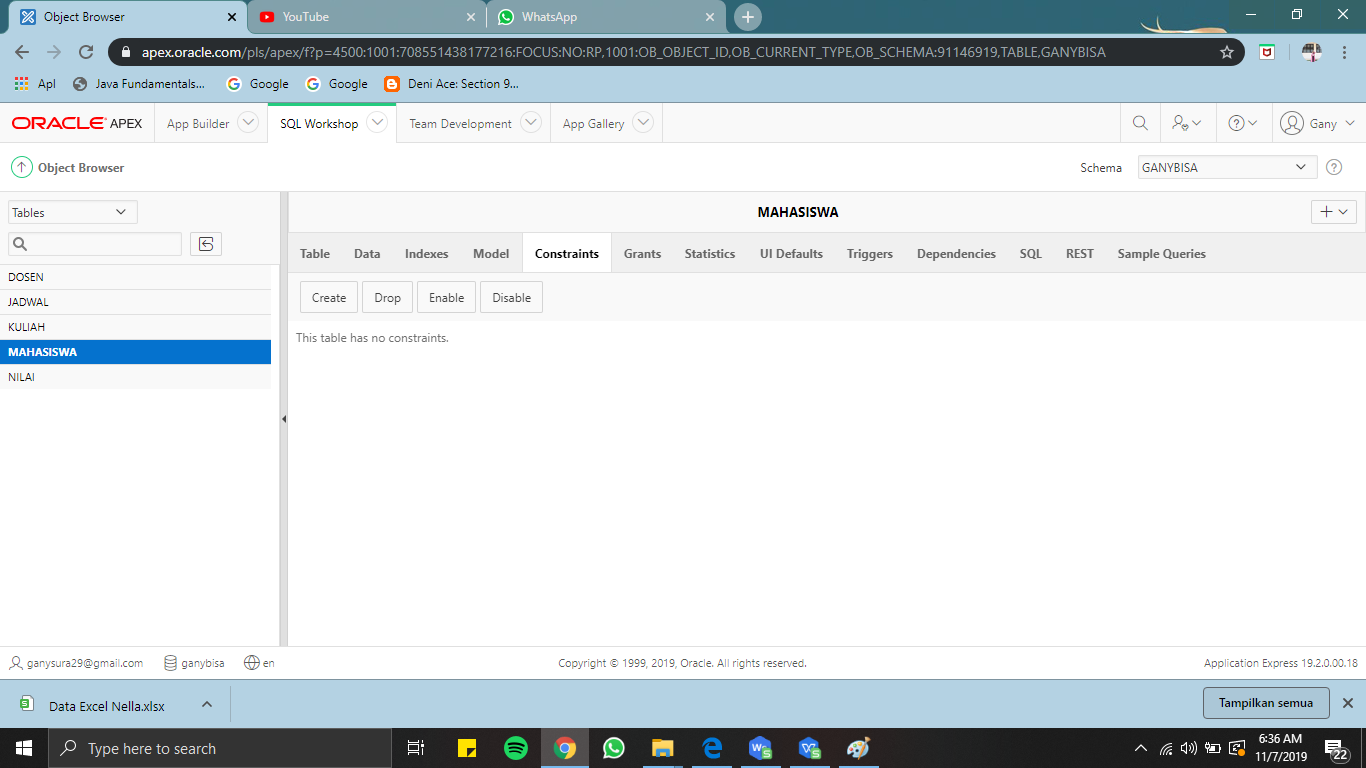
\includegraphics[width=.6\textwidth]{gambar/20.png}
    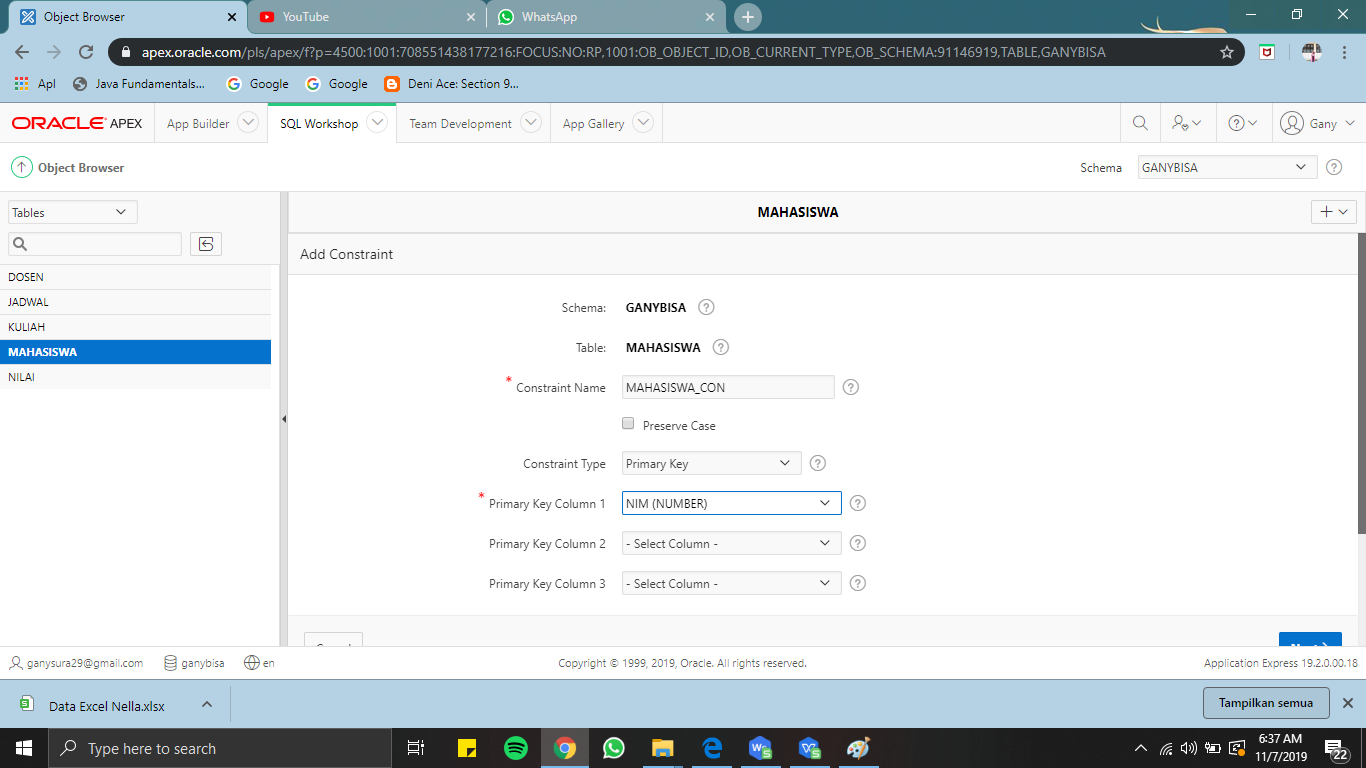
\includegraphics[width=.6\textwidth]{gambar/21.png}
    \end{center}
    \item tabel dosen , CONTAIN TYPE diganti menjadi PRIMARY KEY dan dan pilih tabel NIP, kemudian pilih tombol PLAY dan kita bisa lihat CODINGAN atau SQL yang langsung terbentuk
    \begin{center}
    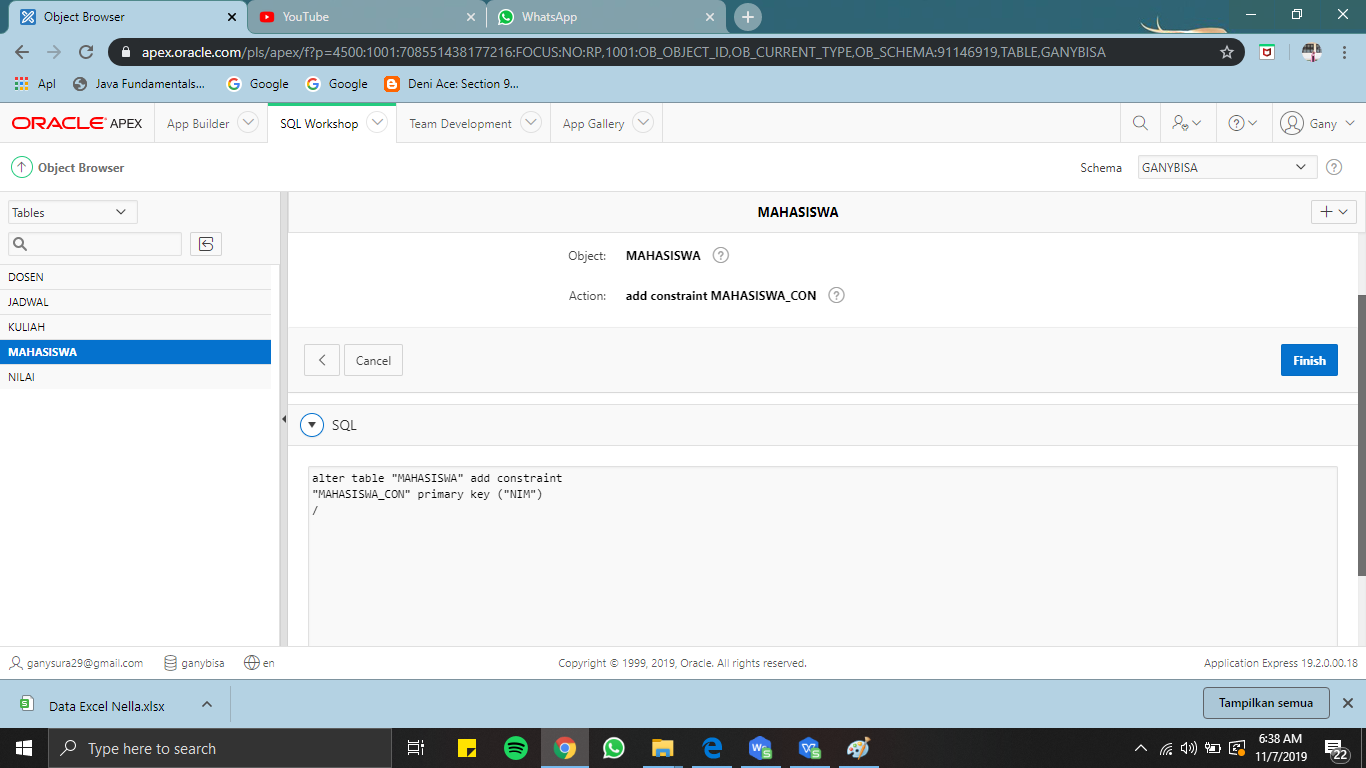
\includegraphics[width=.6\textwidth]{gambar/22.png}
    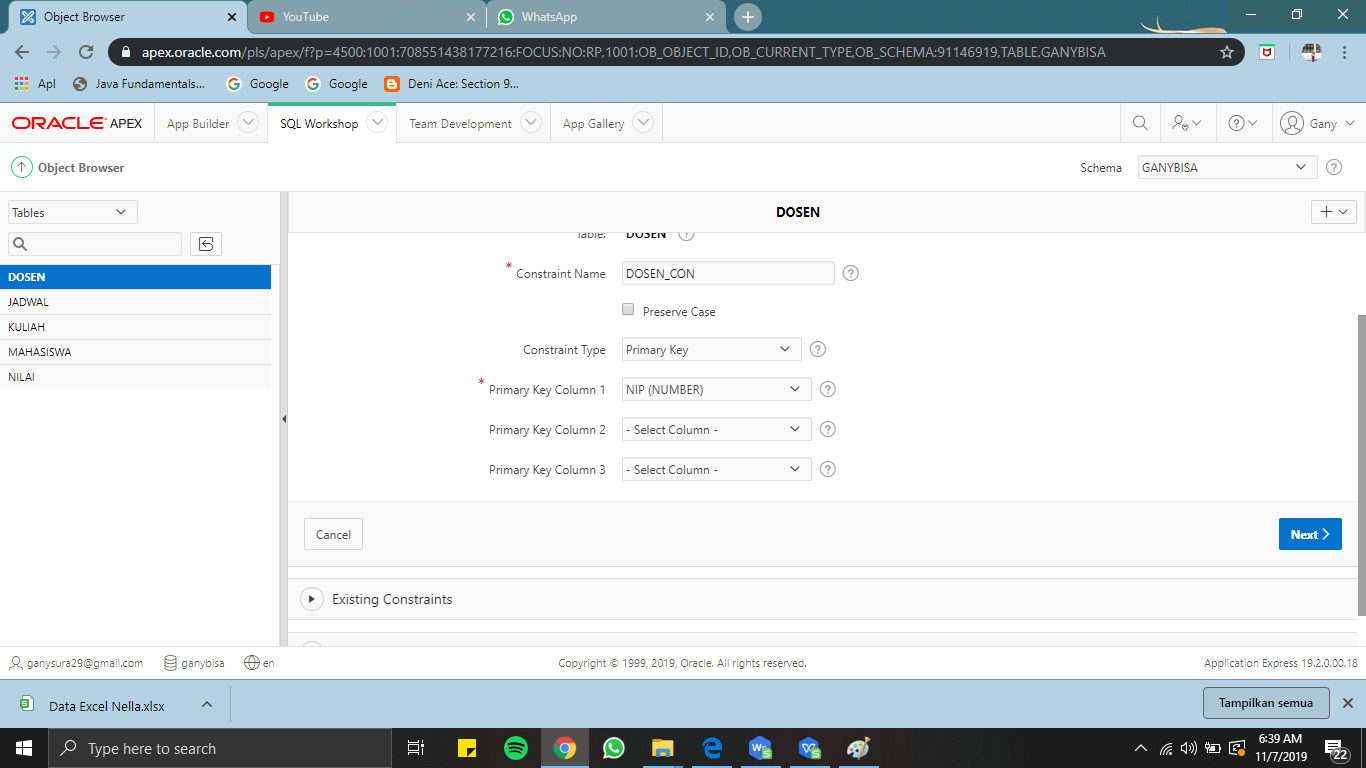
\includegraphics[width=.6\textwidth]{gambar/23.png}
    \end{center}
    \item tabel kuliah , CONTAIN TYPE diganti menjadi PRIMARY KEY dan dan pilih tabel KODE, kemudian pilih tombol PLAY dan kita bisa lihat CODINGAN atau SQL yang langsung terbentuk
    \begin{center}
    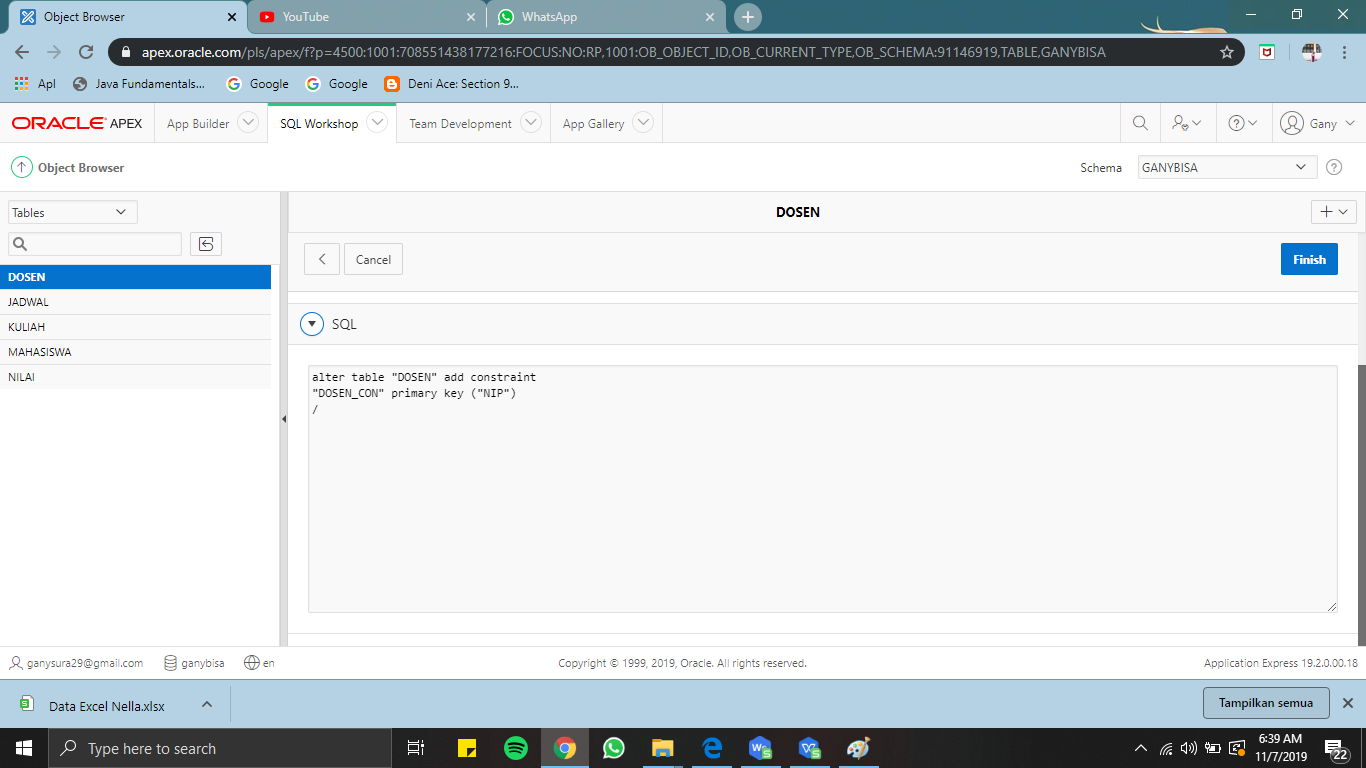
\includegraphics[width=.6\textwidth]{gambar/24.png}
    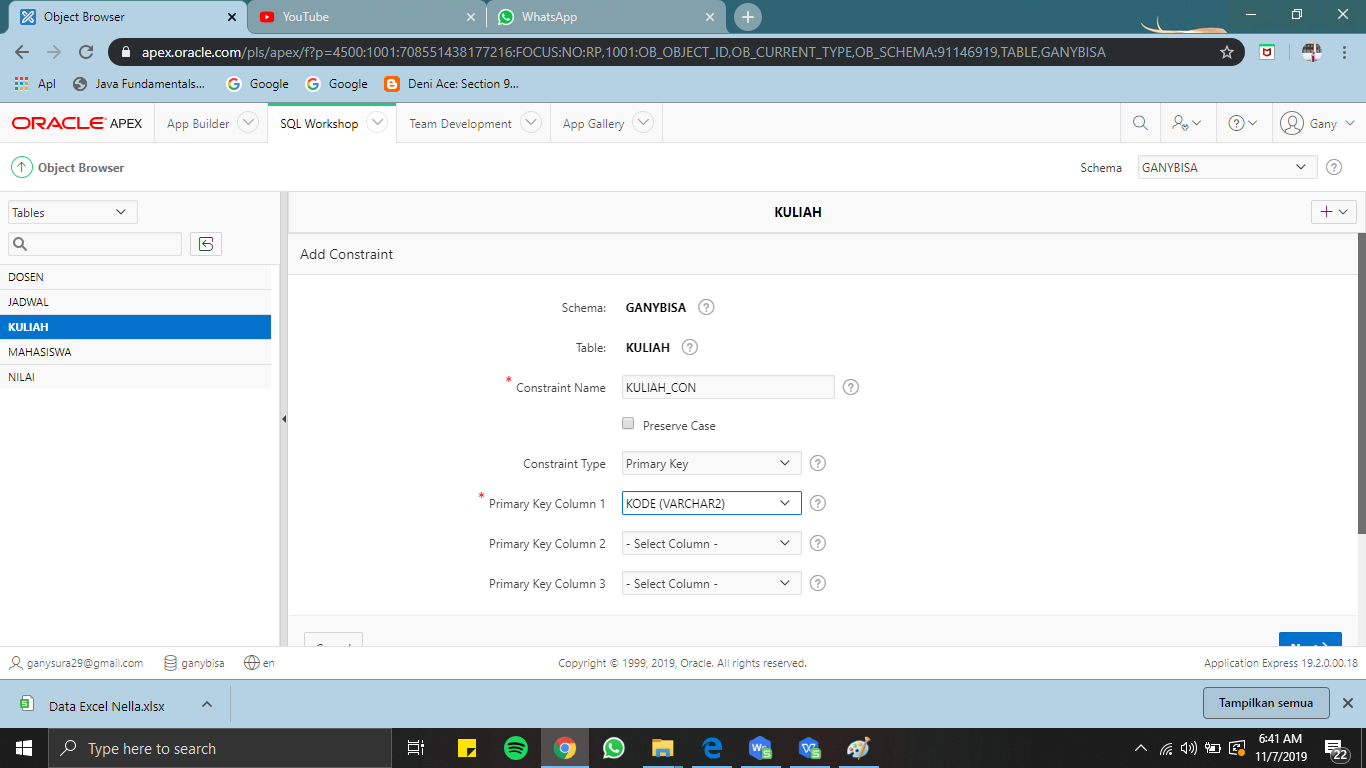
\includegraphics[width=.6\textwidth]{gambar/25.png}
    \end{center}
    \item tabel Jadwal , CONTAIN TYPE diganti menjadi FOREIGN KEY dan dan pilih KODE MATA KULIAH, kemudian buka KULIAH dan klik KODE , kemudian pilih tombol PLAY dan kita bisa lihat CODINGAN atau SQL yang langsung terbentuk
    \begin{center}
    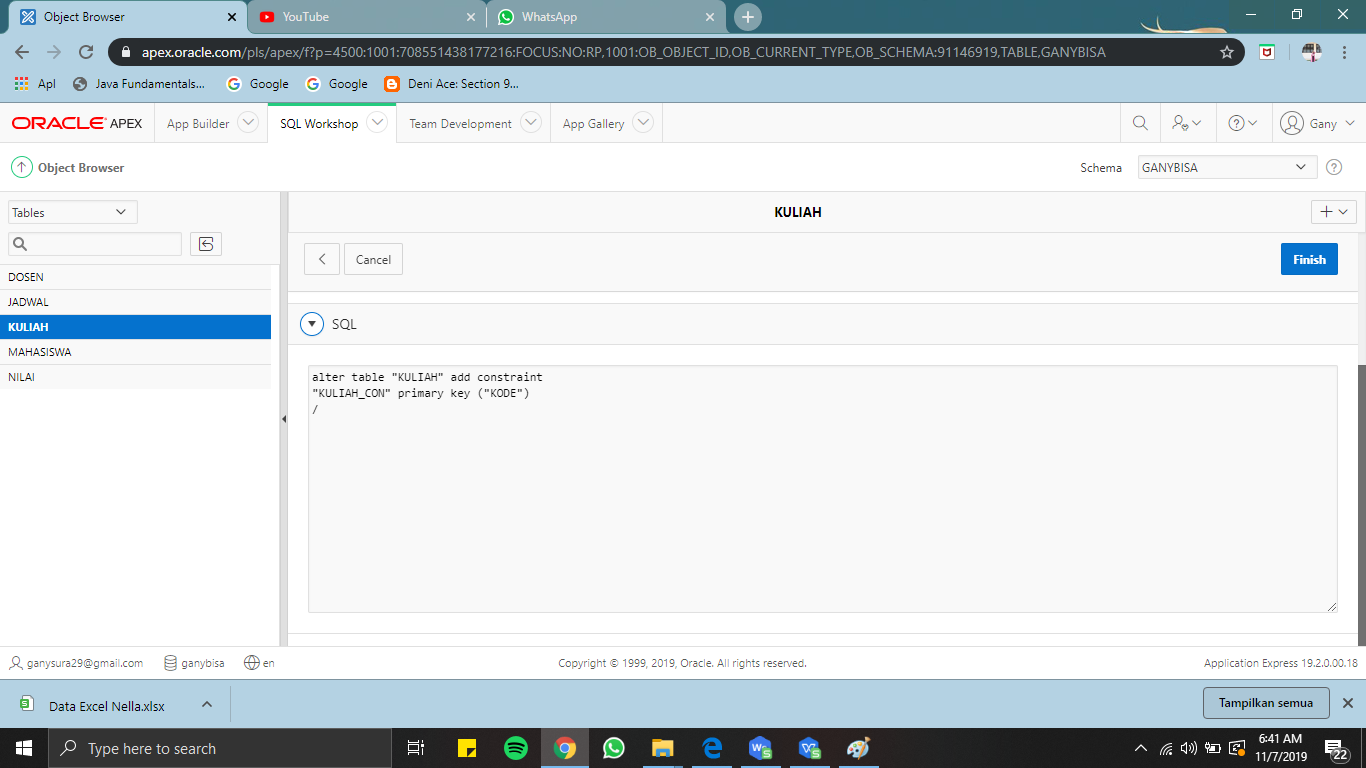
\includegraphics[width=.6\textwidth]{gambar/26.png}
    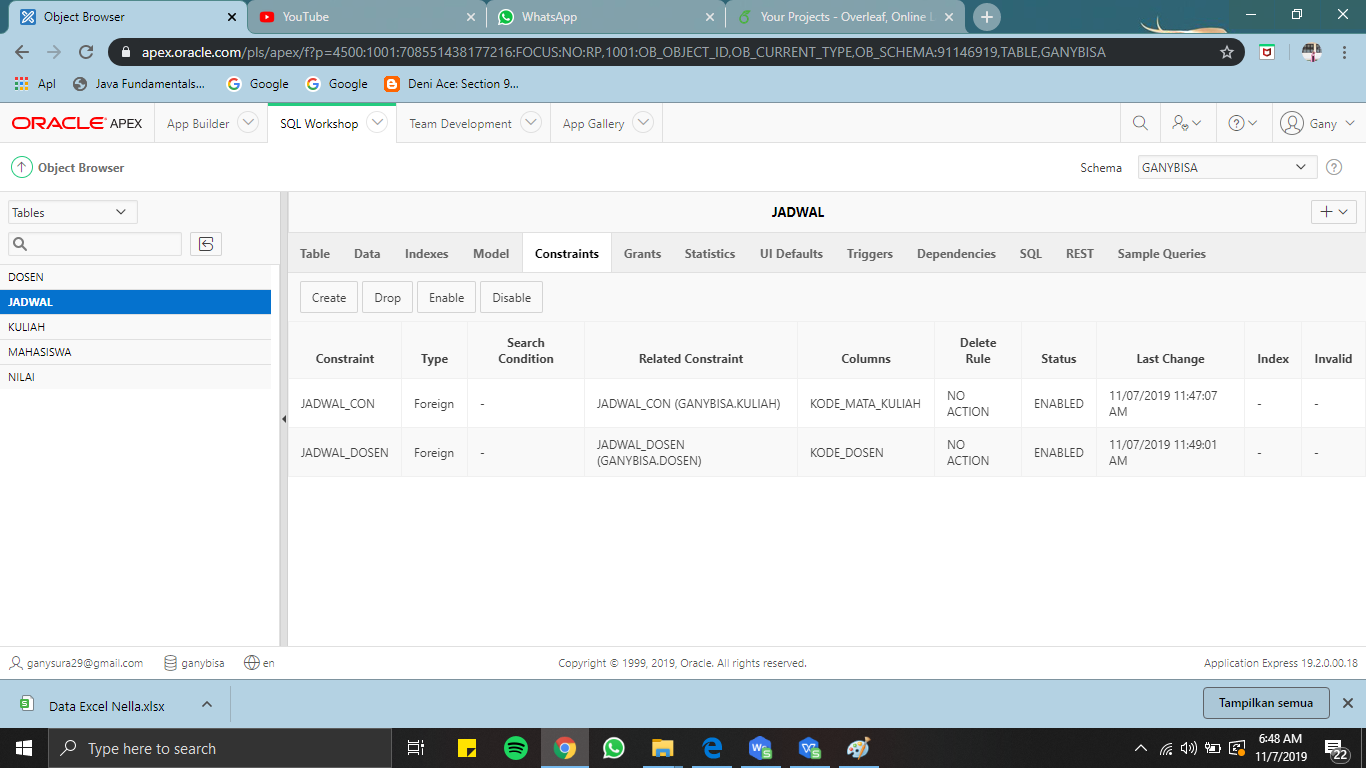
\includegraphics[width=.6\textwidth]{gambar/31.png}
    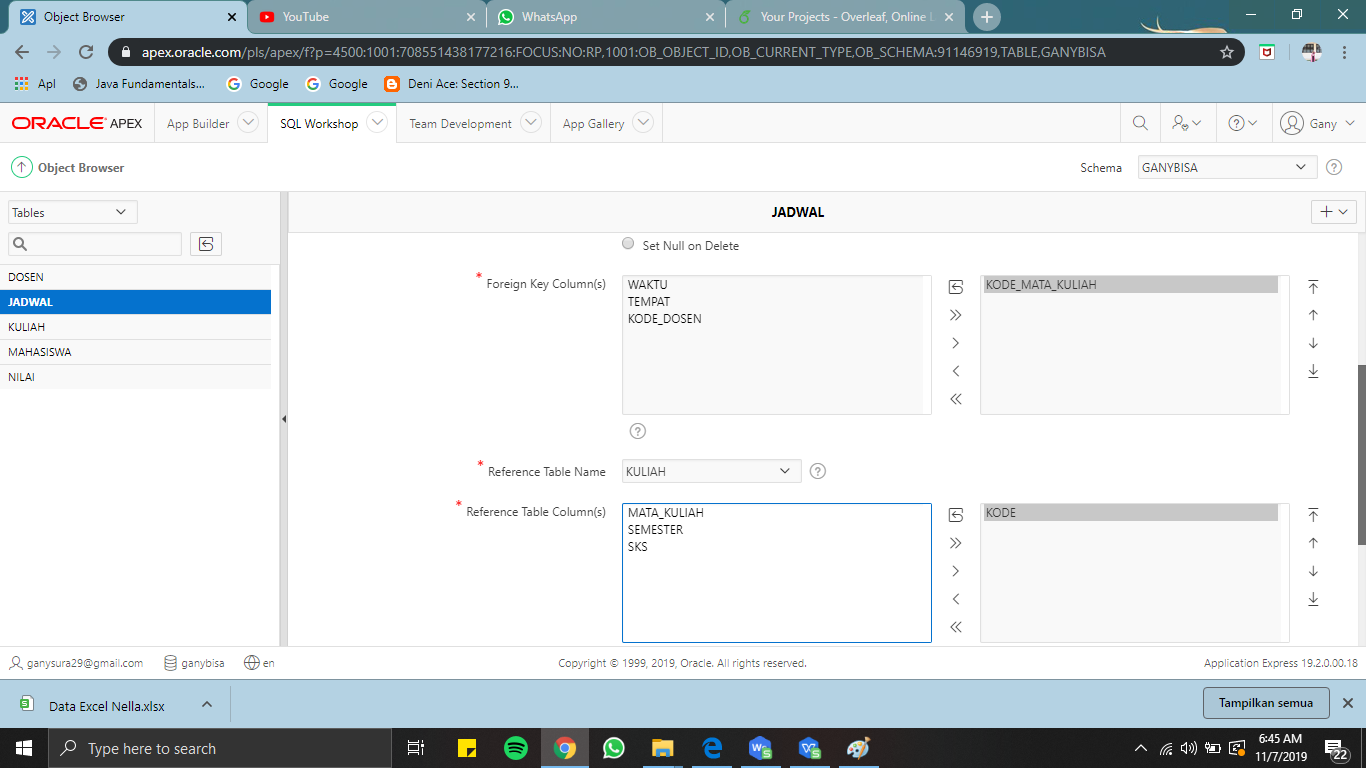
\includegraphics[width=.6\textwidth]{gambar/27.png}
    \end{center}
    \item lakukan pada tabel NILAI , CONTAIN TYPE diganti menjadi FOREIGN KEY dan dan pilih NIM, kemudian buka MAHASISWA dan klik NIM , kemudian pilih tombol PLAY dan kita bisa lihat CODINGAN atau SQL yang langsung terbentuk
    \begin{center}
    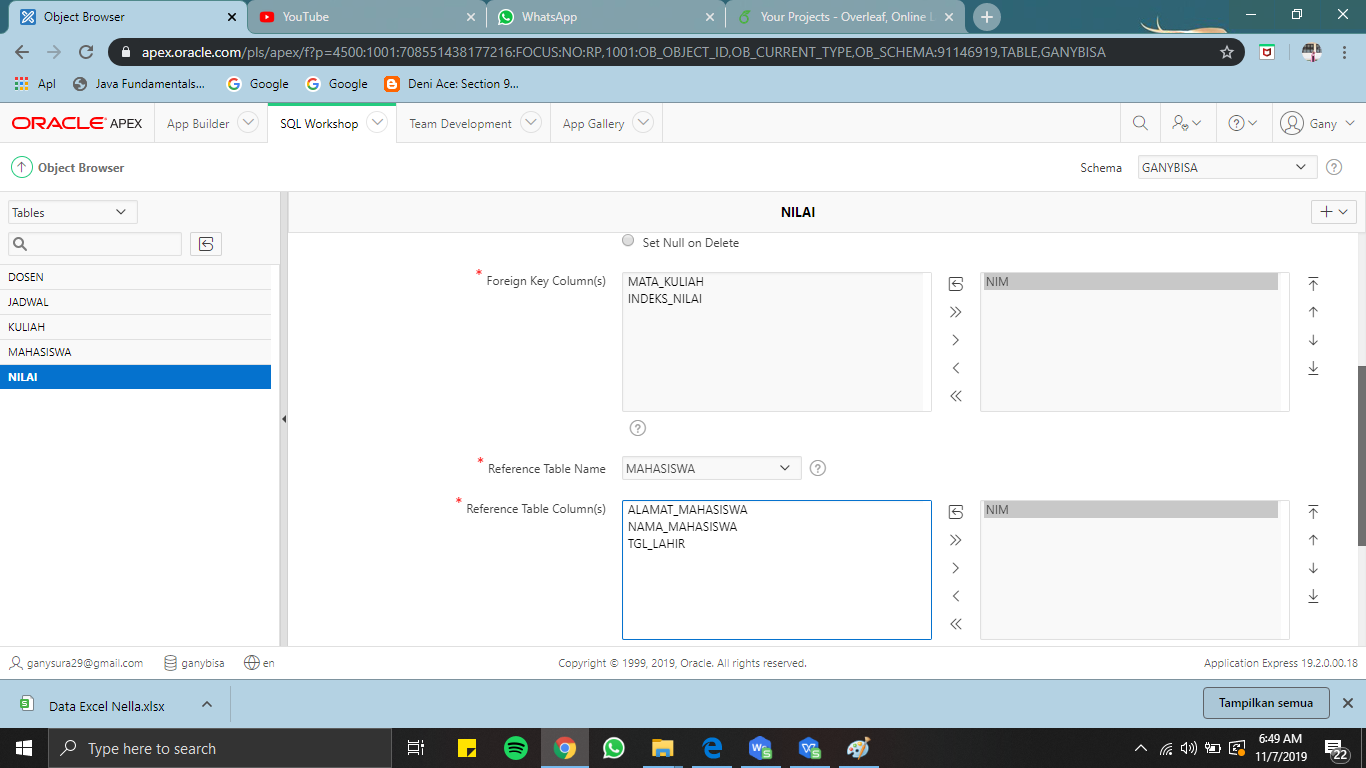
\includegraphics[width=.6\textwidth]{gambar/32.png}
    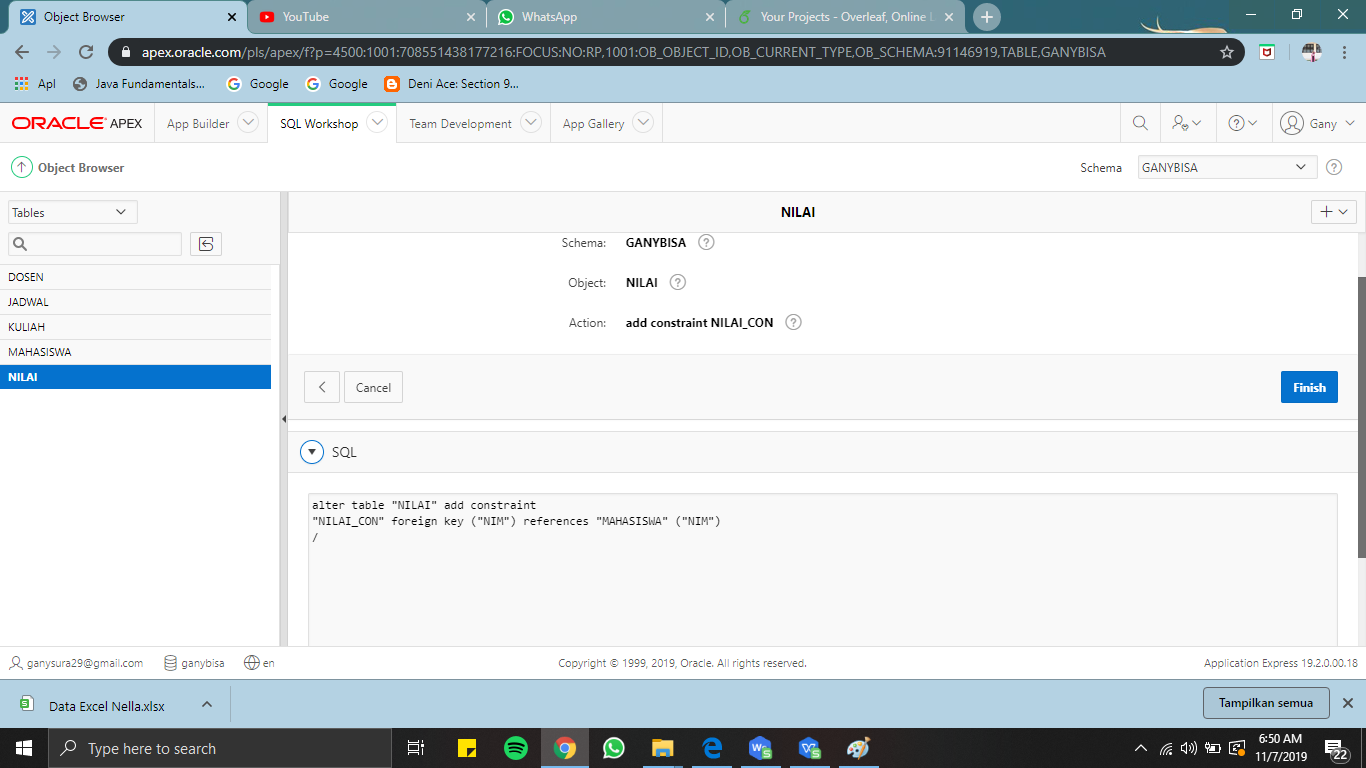
\includegraphics[width=.6\textwidth]{gambar/33.png}
    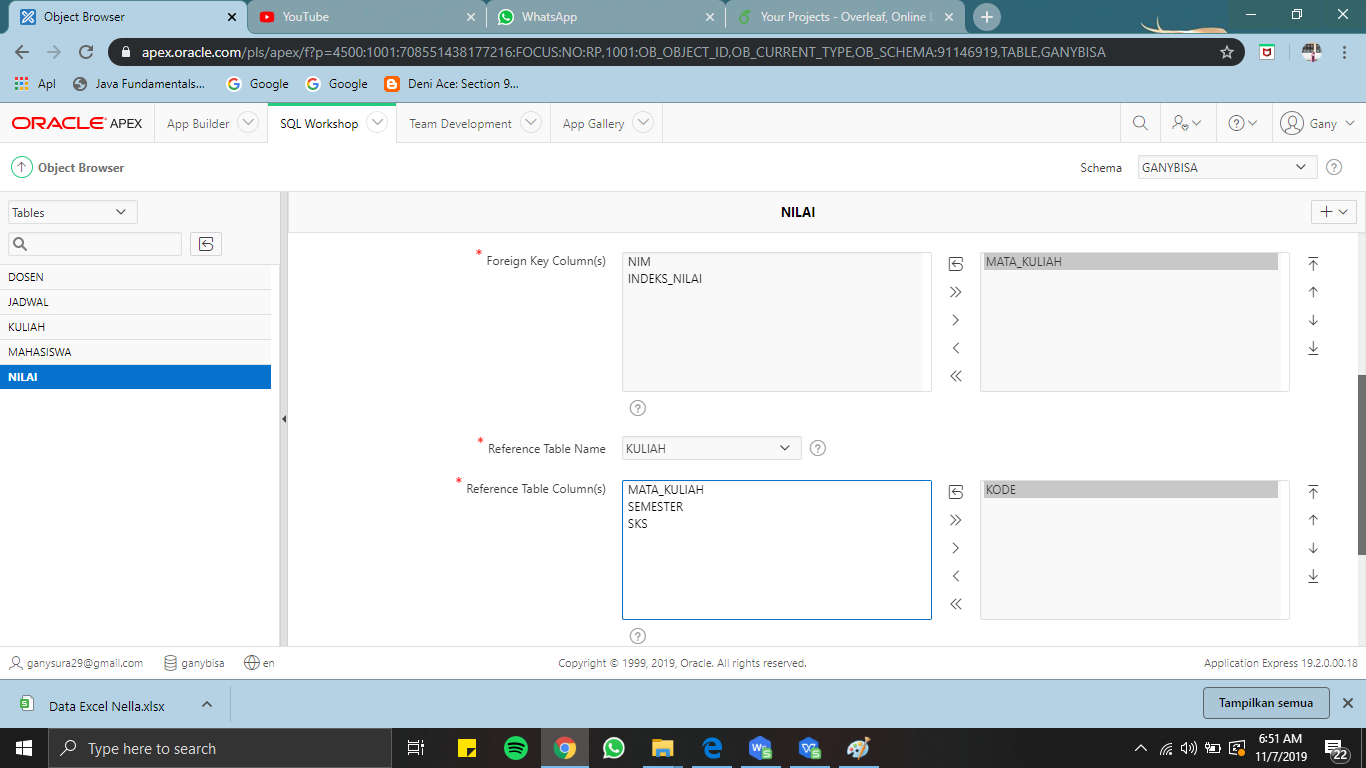
\includegraphics[width=.6\textwidth]{gambar/34.png}
    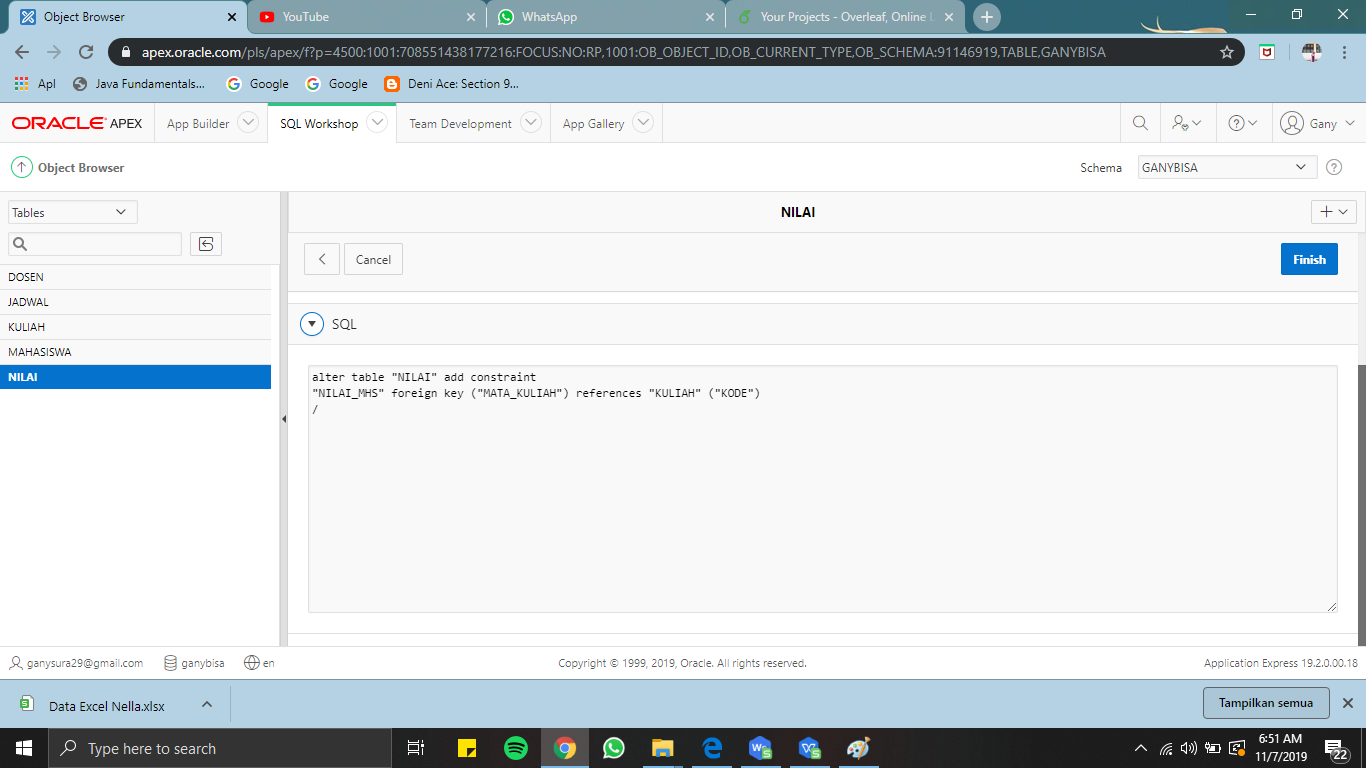
\includegraphics[width=.6\textwidth]{gambar/35.png}
    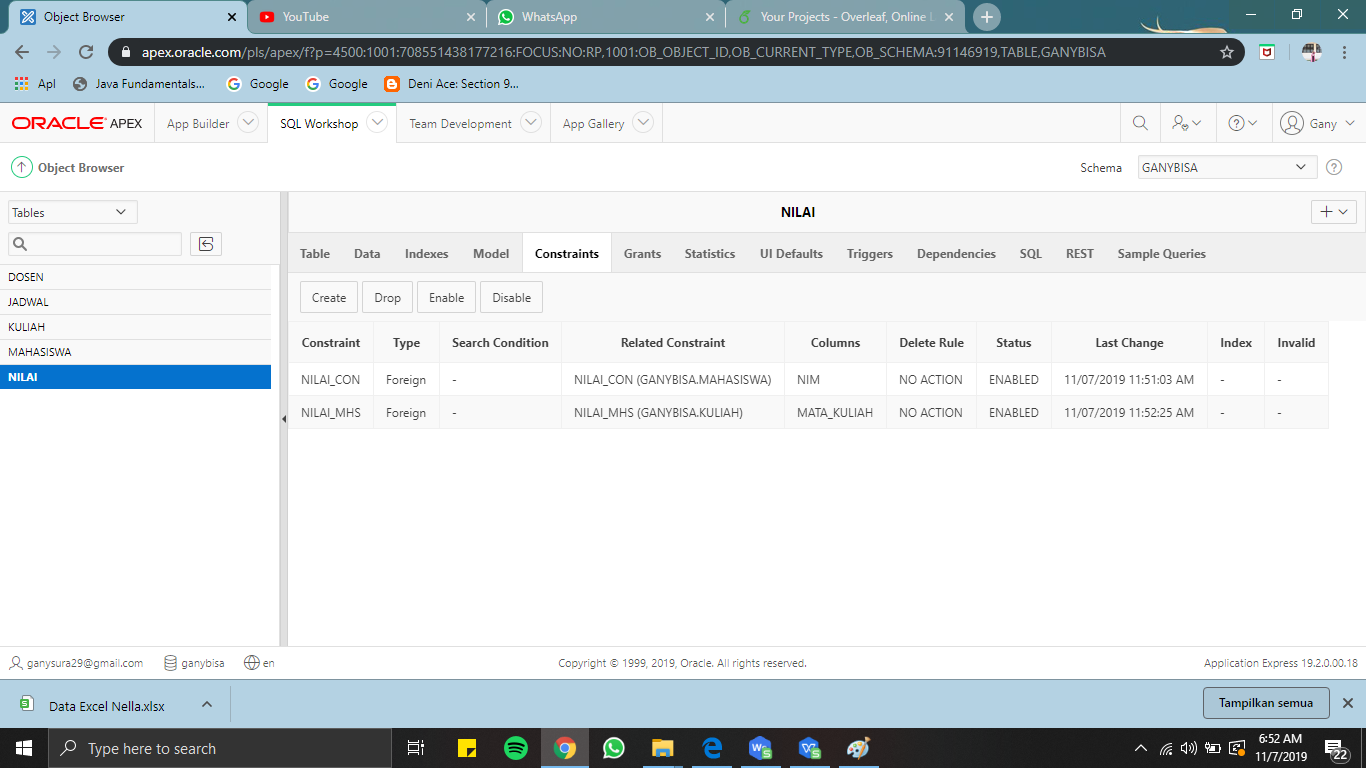
\includegraphics[width=.6\textwidth]{gambar/36.png}
    \end{center}
    \item kemudian balik lagi ke menu awal dan dan pilih CREATE kemudian pilih NEW APLICATION
     \begin{center}
    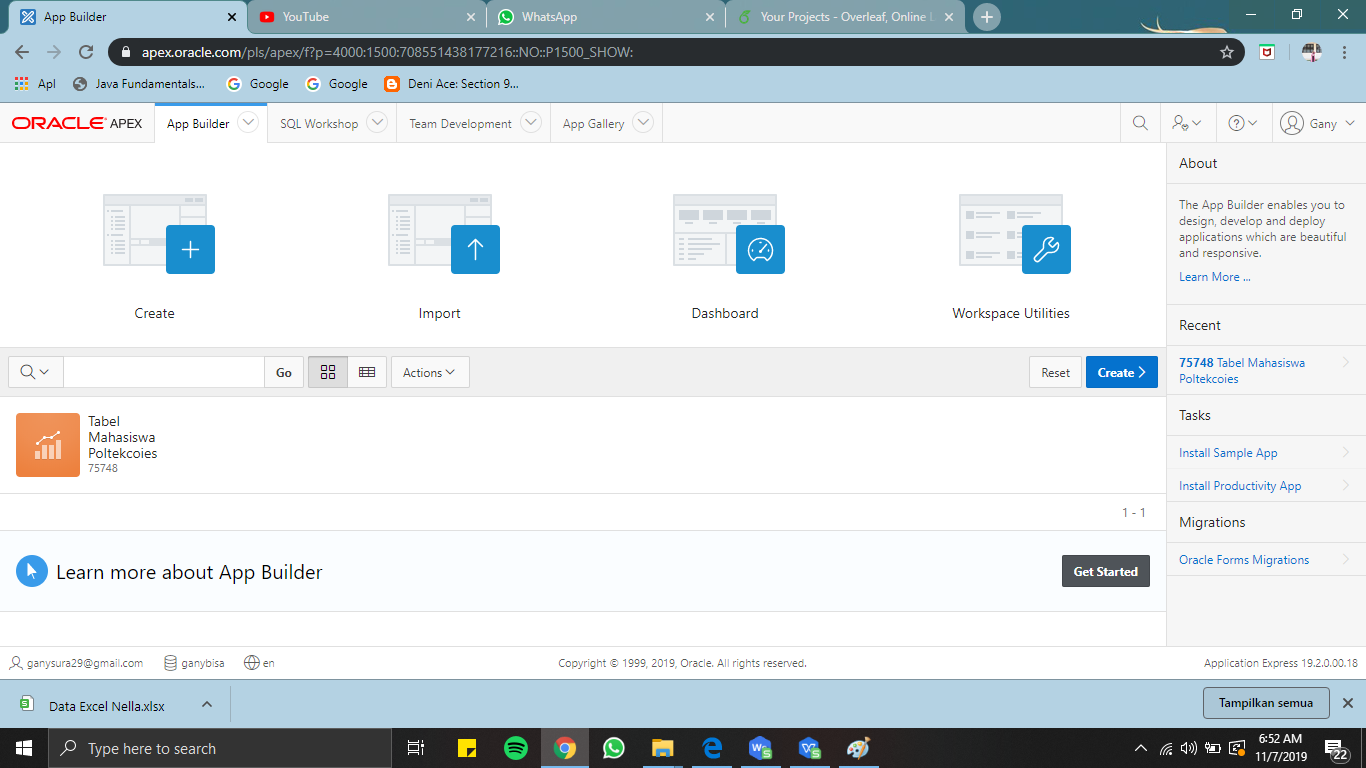
\includegraphics[width=.6\textwidth]{gambar/37.png}
    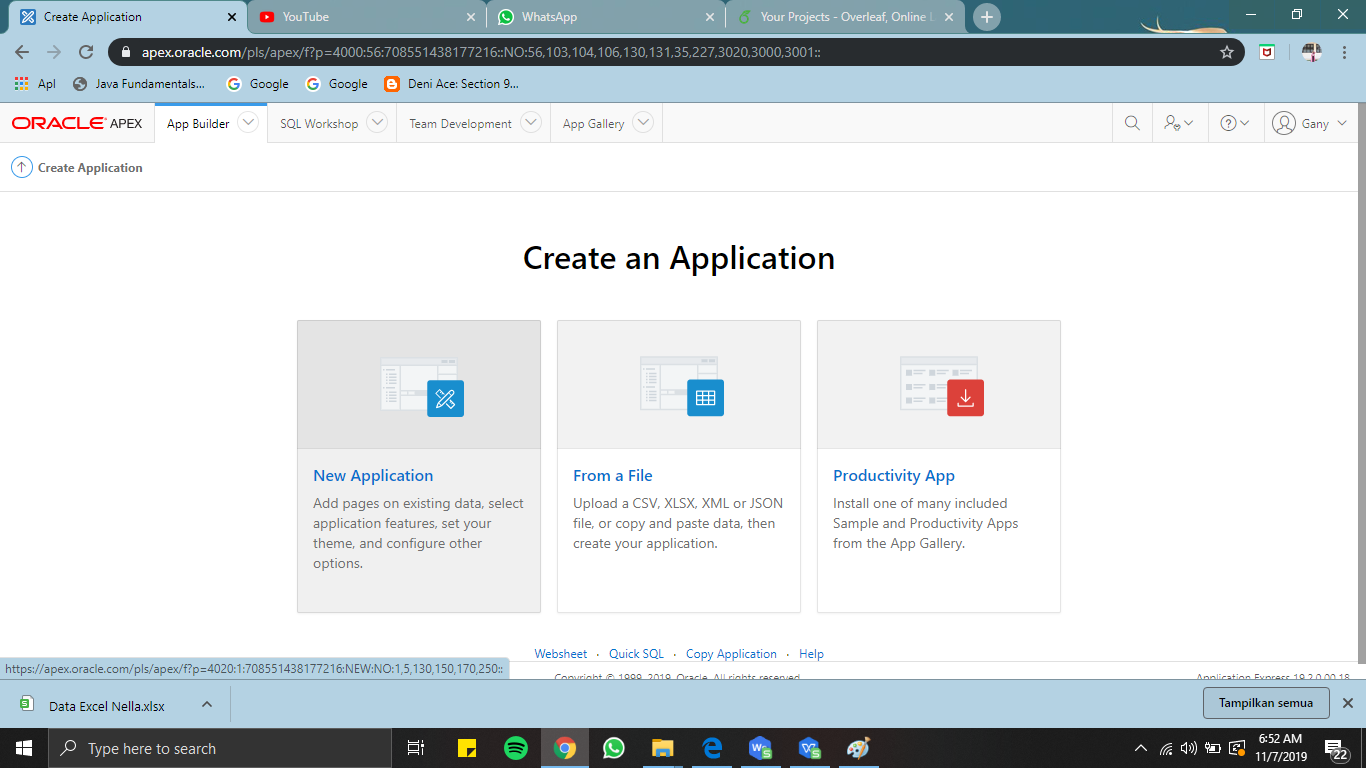
\includegraphics[width=.6\textwidth]{gambar/38.png}
    \end{center}
    \item pilih ADD PAGE, kemudian pilih INTERAKTIVE REPORT, dan rubah nama menjadi nama tabel yang telah dibuat yaitu MAHASISWA, hingga JADWAL
     \begin{center}
    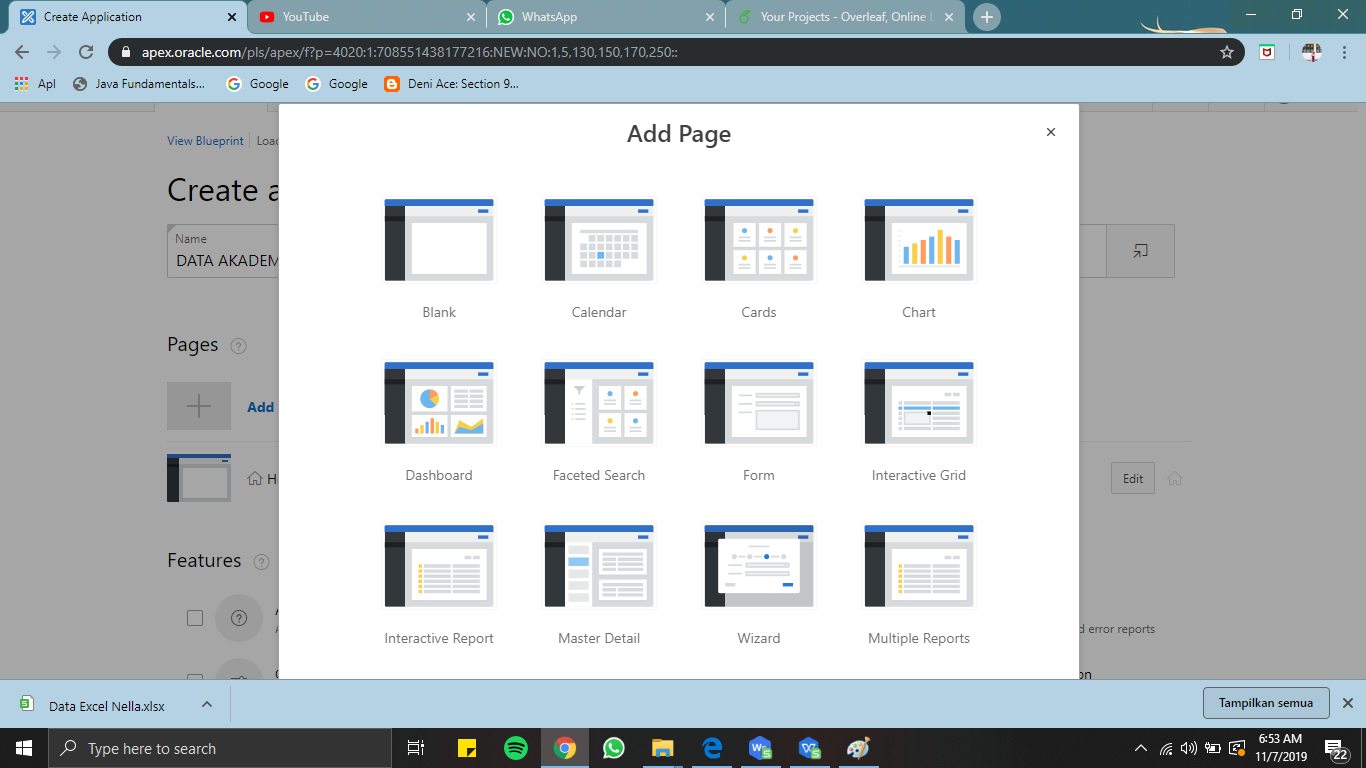
\includegraphics[width=.6\textwidth]{gambar/39.png}
    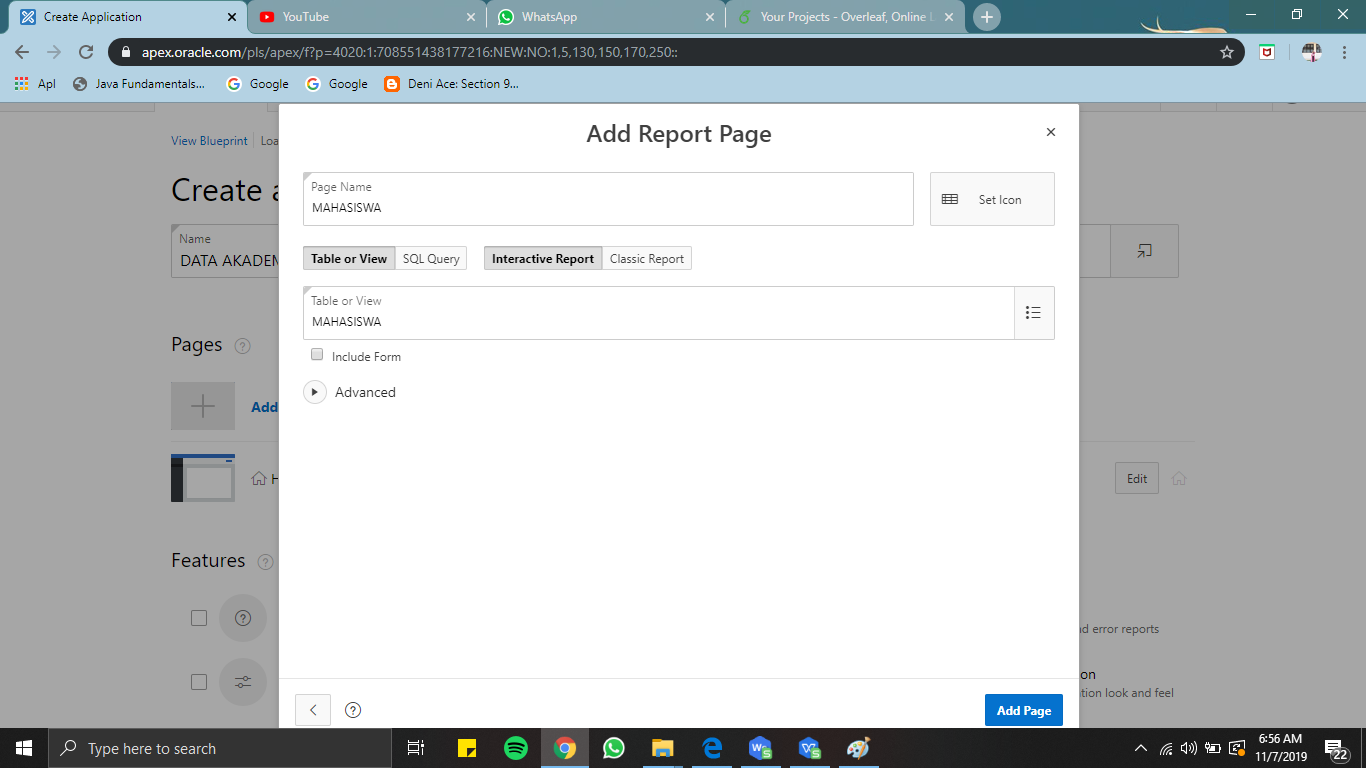
\includegraphics[width=.6\textwidth]{gambar/40.png}
    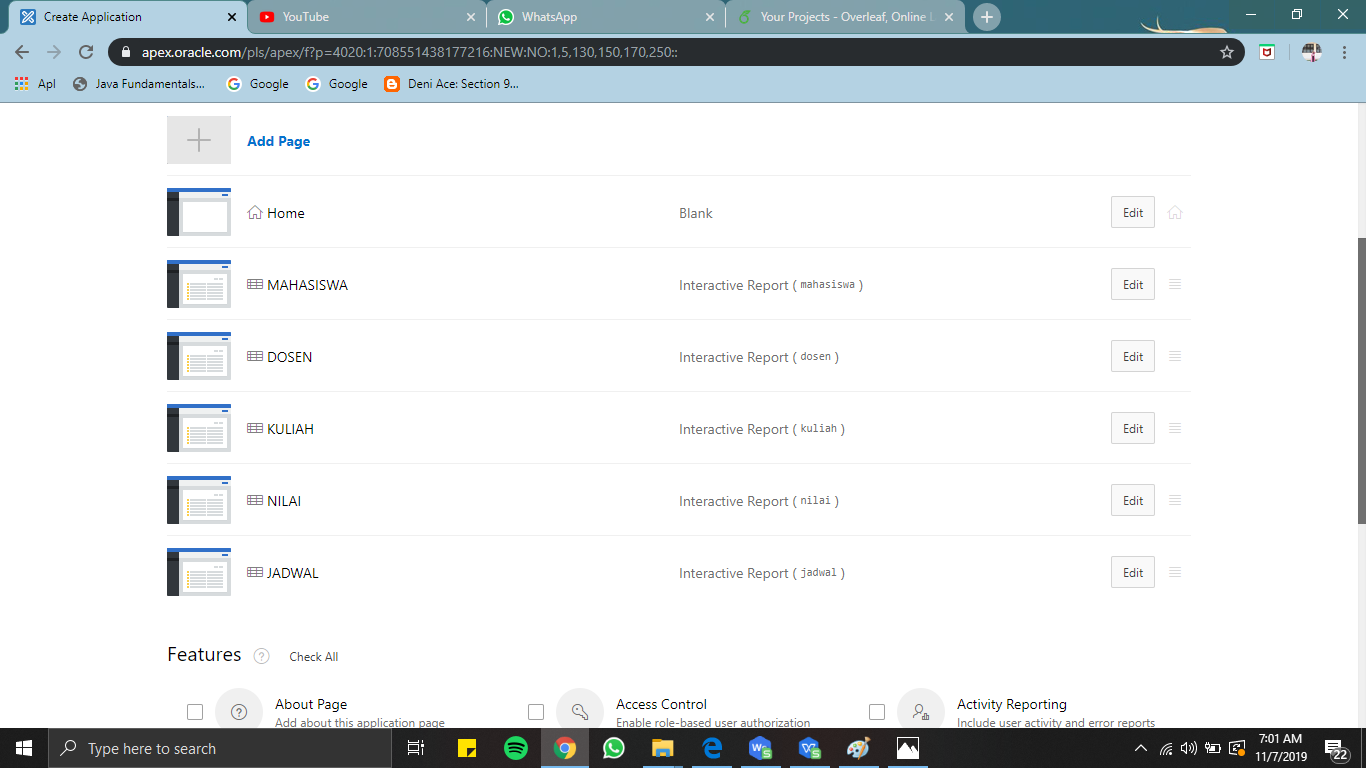
\includegraphics[width=.6\textwidth]{gambar/41.png}
    \end{center}
    \item setelah itu RUN APPLICATION
    \begin{center}
    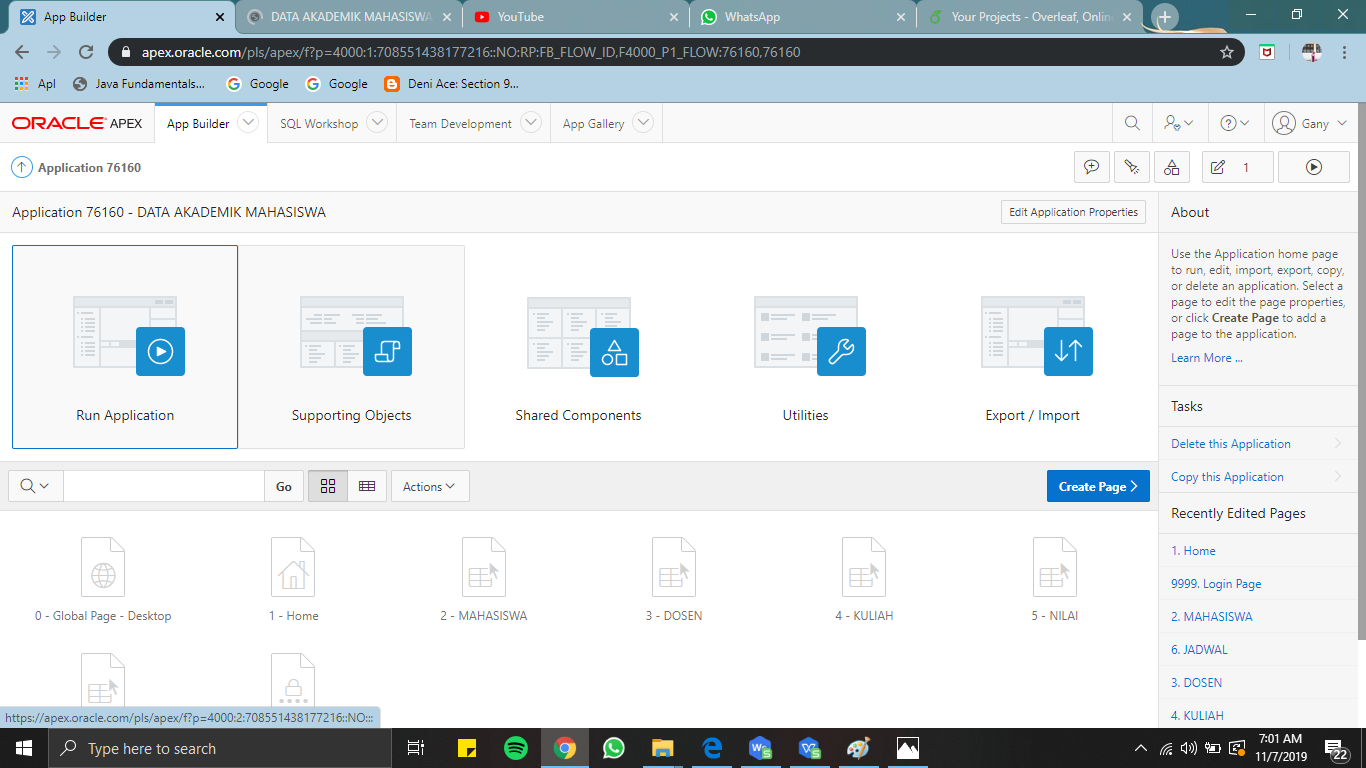
\includegraphics[width=.6\textwidth]{gambar/42.png}
    \end{center}
    \item Login dengan user name serta password, USERNAME : GANYSURA29@GMAIL.COM dengan PASSWORD : Tujuhbelasjuni2000
    \item https://apex.oracle.com/pls/apex/f?p=76160:LOGIN_DESKTOP:122683758485081:::::
    \begin{center}
    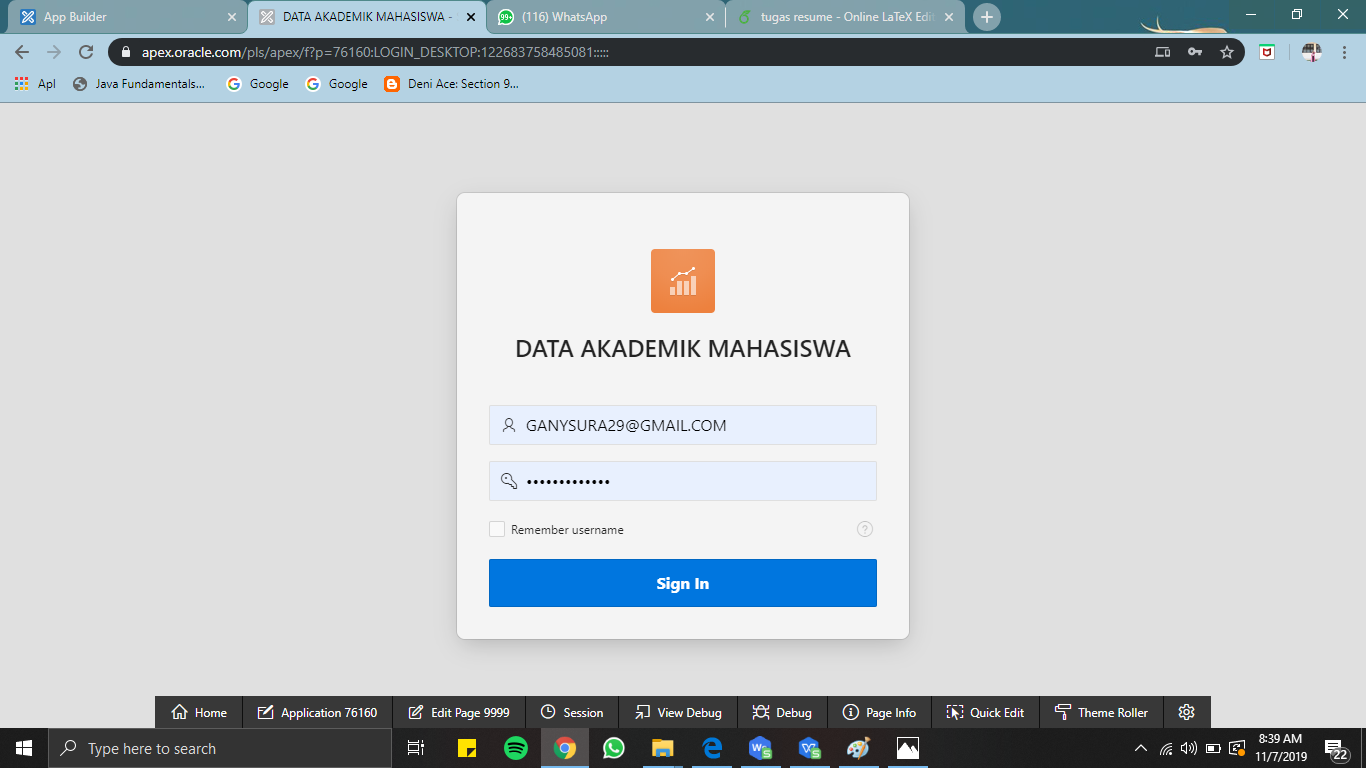
\includegraphics[width=.6\textwidth]{gambar/46.png}
    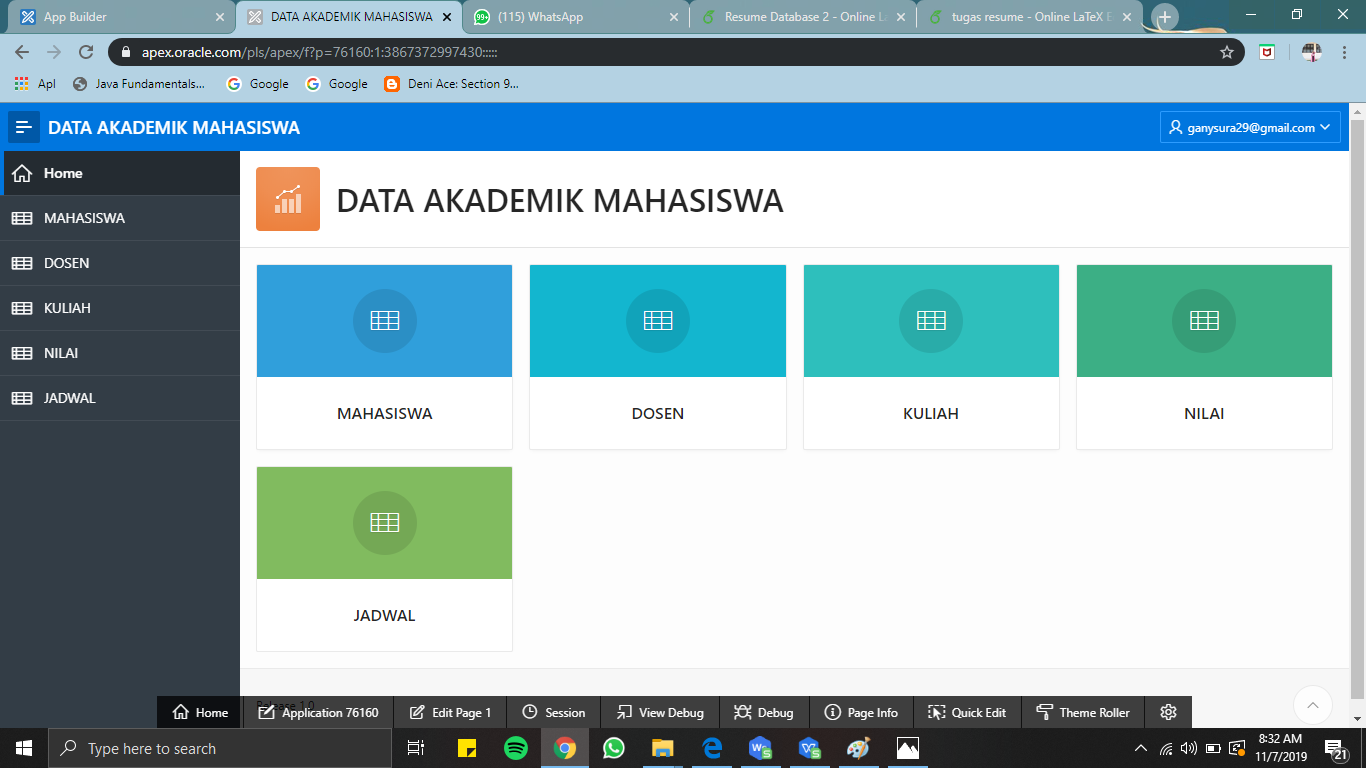
\includegraphics[width=.6\textwidth]{gambar/45.png}
    \end{center}
\end{enumerate}

\end{document}
